\documentclass[12pt]{article}
\usepackage{tocloft}
\usepackage{url}
\usepackage[utf8x]{inputenc}
\usepackage{amsmath}
\usepackage{graphicx}
\usepackage{verbatim}
\graphicspath{{images/}}
\usepackage{parskip}
\usepackage{fancyhdr}
\usepackage{vmargin}
\setmarginsrb{3 cm}{2.5 cm}{3 cm}{2.5 cm}{1 cm}{1.5 cm}{1 cm}{1.5 cm}
\usepackage{appendix}
\usepackage{listings} % For code importing
\usepackage{xcolor} % for setting colors
\usepackage{biblatex}
\addbibresource{ref.bib}
 %%%%%%%%%%%%%%%%%%%%%%%%%%%%%%%%%%%%%%%%%%%%%%%%%%%%%%%%%%%%%%%%%%%%%%%%%%%%%%%% 
%%% ~ Arduino Language - Arduino IDE Colors ~                                  %%%
%%%                                                                            %%%
%%% Kyle Rocha-Brownell | 10/2/2017 | No Licence                               %%%
%%% -------------------------------------------------------------------------- %%%
%%%                                                                            %%%
%%% Place this file in your working directory (next to the latex file you're   %%%
%%% working on).  To add it to your project, place:                            %%%
%%%     %%%%%%%%%%%%%%%%%%%%%%%%%%%%%%%%%%%%%%%%%%%%%%%%%%%%%%%%%%%%%%%%%%%%%%%%%%%%%%%% 
%%% ~ Arduino Language - Arduino IDE Colors ~                                  %%%
%%%                                                                            %%%
%%% Kyle Rocha-Brownell | 10/2/2017 | No Licence                               %%%
%%% -------------------------------------------------------------------------- %%%
%%%                                                                            %%%
%%% Place this file in your working directory (next to the latex file you're   %%%
%%% working on).  To add it to your project, place:                            %%%
%%%     %%%%%%%%%%%%%%%%%%%%%%%%%%%%%%%%%%%%%%%%%%%%%%%%%%%%%%%%%%%%%%%%%%%%%%%%%%%%%%%% 
%%% ~ Arduino Language - Arduino IDE Colors ~                                  %%%
%%%                                                                            %%%
%%% Kyle Rocha-Brownell | 10/2/2017 | No Licence                               %%%
%%% -------------------------------------------------------------------------- %%%
%%%                                                                            %%%
%%% Place this file in your working directory (next to the latex file you're   %%%
%%% working on).  To add it to your project, place:                            %%%
%%%    \input{arduinoLanguage.tex}                                             %%%
%%% somewhere before \begin{document} in your latex file.                      %%%
%%%                                                                            %%%
%%% In your document, place your arduino code between:                         %%%
%%%   \begin{lstlisting}[language=Arduino]                                     %%%
%%% and:                                                                       %%%
%%%   \end{lstlisting}                                                         %%%
%%%                                                                            %%%
%%% Or create your own style to add non-built-in functions and variables.      %%%
%%%                                                                            %%%
 %%%%%%%%%%%%%%%%%%%%%%%%%%%%%%%%%%%%%%%%%%%%%%%%%%%%%%%%%%%%%%%%%%%%%%%%%%%%%%%% 

\usepackage{color}
\usepackage{listings}    
\usepackage{courier}

%%% Define Custom IDE Colors %%%
\definecolor{arduinoGreen}    {rgb} {0.17, 0.43, 0.01}
\definecolor{arduinoGrey}     {rgb} {0.47, 0.47, 0.33}
\definecolor{arduinoOrange}   {rgb} {0.8 , 0.4 , 0   }
\definecolor{arduinoBlue}     {rgb} {0.01, 0.61, 0.98}
\definecolor{arduinoDarkBlue} {rgb} {0.0 , 0.2 , 0.5 }

%%% Define Arduino Language %%%
\lstdefinelanguage{Arduino}{
  language=C++, % begin with default C++ settings 
%
%
  %%% Keyword Color Group 1 %%%  (called KEYWORD3 by arduino)
  keywordstyle=\color{arduinoGreen},   
  deletekeywords={  % remove all arduino keywords that might be in c++
                break, case, override, final, continue, default, do, else, for, 
                if, return, goto, switch, throw, try, while, setup, loop, export, 
                not, or, and, xor, include, define, elif, else, error, if, ifdef, 
                ifndef, pragma, warning,
                HIGH, LOW, INPUT, INPUT_PULLUP, OUTPUT, DEC, BIN, HEX, OCT, PI, 
                HALF_PI, TWO_PI, LSBFIRST, MSBFIRST, CHANGE, FALLING, RISING, 
                DEFAULT, EXTERNAL, INTERNAL, INTERNAL1V1, INTERNAL2V56, LED_BUILTIN, 
                LED_BUILTIN_RX, LED_BUILTIN_TX, DIGITAL_MESSAGE, FIRMATA_STRING, 
                ANALOG_MESSAGE, REPORT_DIGITAL, REPORT_ANALOG, SET_PIN_MODE, 
                SYSTEM_RESET, SYSEX_START, auto, int8_t, int16_t, int32_t, int64_t, 
                uint8_t, uint16_t, uint32_t, uint64_t, char16_t, char32_t, operator, 
                enum, delete, bool, boolean, byte, char, const, false, float, double, 
                null, NULL, int, long, new, private, protected, public, short, 
                signed, static, volatile, String, void, true, unsigned, word, array, 
                sizeof, dynamic_cast, typedef, const_cast, struct, static_cast, union, 
                friend, extern, class, reinterpret_cast, register, explicit, inline, 
                _Bool, complex, _Complex, _Imaginary, atomic_bool, atomic_char, 
                atomic_schar, atomic_uchar, atomic_short, atomic_ushort, atomic_int, 
                atomic_uint, atomic_long, atomic_ulong, atomic_llong, atomic_ullong, 
                virtual, PROGMEM,
                Serial, Serial1, Serial2, Serial3, SerialUSB, Keyboard, Mouse,
                abs, acos, asin, atan, atan2, ceil, constrain, cos, degrees, exp, 
                floor, log, map, max, min, radians, random, randomSeed, round, sin, 
                sq, sqrt, tan, pow, bitRead, bitWrite, bitSet, bitClear, bit, 
                highByte, lowByte, analogReference, analogRead, 
                analogReadResolution, analogWrite, analogWriteResolution, 
                attachInterrupt, detachInterrupt, digitalPinToInterrupt, delay, 
                delayMicroseconds, digitalWrite, digitalRead, interrupts, millis, 
                micros, noInterrupts, noTone, pinMode, pulseIn, pulseInLong, shiftIn, 
                shiftOut, tone, yield, Stream, begin, end, peek, read, print, 
                println, available, availableForWrite, flush, setTimeout, find, 
                findUntil, parseInt, parseFloat, readBytes, readBytesUntil, readString, 
                readStringUntil, trim, toUpperCase, toLowerCase, charAt, compareTo, 
                concat, endsWith, startsWith, equals, equalsIgnoreCase, getBytes, 
                indexOf, lastIndexOf, length, replace, setCharAt, substring, 
                toCharArray, toInt, press, release, releaseAll, accept, click, move, 
                isPressed, isAlphaNumeric, isAlpha, isAscii, isWhitespace, isControl, 
                isDigit, isGraph, isLowerCase, isPrintable, isPunct, isSpace, 
                isUpperCase, isHexadecimalDigit, 
                }, 
  morekeywords={   % add arduino structures to group 1
                break, case, override, final, continue, default, do, else, for, 
                if, return, goto, switch, throw, try, while, setup, loop, export, 
                not, or, and, xor, include, define, elif, else, error, if, ifdef, 
                ifndef, pragma, warning,
                }, 
% 
%
  %%% Keyword Color Group 2 %%%  (called LITERAL1 by arduino)
  keywordstyle=[2]\color{arduinoBlue},   
  keywords=[2]{   % add variables and dataTypes as 2nd group  
                HIGH, LOW, INPUT, INPUT_PULLUP, OUTPUT, DEC, BIN, HEX, OCT, PI, 
                HALF_PI, TWO_PI, LSBFIRST, MSBFIRST, CHANGE, FALLING, RISING, 
                DEFAULT, EXTERNAL, INTERNAL, INTERNAL1V1, INTERNAL2V56, LED_BUILTIN, 
                LED_BUILTIN_RX, LED_BUILTIN_TX, DIGITAL_MESSAGE, FIRMATA_STRING, 
                ANALOG_MESSAGE, REPORT_DIGITAL, REPORT_ANALOG, SET_PIN_MODE, 
                SYSTEM_RESET, SYSEX_START, auto, int8_t, int16_t, int32_t, int64_t, 
                uint8_t, uint16_t, uint32_t, uint64_t, char16_t, char32_t, operator, 
                enum, delete, bool, boolean, byte, char, const, false, float, double, 
                null, NULL, int, long, new, private, protected, public, short, 
                signed, static, volatile, String, void, true, unsigned, word, array, 
                sizeof, dynamic_cast, typedef, const_cast, struct, static_cast, union, 
                friend, extern, class, reinterpret_cast, register, explicit, inline, 
                _Bool, complex, _Complex, _Imaginary, atomic_bool, atomic_char, 
                atomic_schar, atomic_uchar, atomic_short, atomic_ushort, atomic_int, 
                atomic_uint, atomic_long, atomic_ulong, atomic_llong, atomic_ullong, 
                virtual, PROGMEM,
                },  
% 
%
  %%% Keyword Color Group 3 %%%  (called KEYWORD1 by arduino)
  keywordstyle=[3]\bfseries\color{arduinoOrange},
  keywords=[3]{  % add built-in functions as a 3rd group
                Serial, Serial1, Serial2, Serial3, SerialUSB, Keyboard, Mouse,
                },      
%
%
  %%% Keyword Color Group 4 %%%  (called KEYWORD2 by arduino)
  keywordstyle=[4]\color{arduinoOrange},
  keywords=[4]{  % add more built-in functions as a 4th group
                abs, acos, asin, atan, atan2, ceil, constrain, cos, degrees, exp, 
                floor, log, map, max, min, radians, random, randomSeed, round, sin, 
                sq, sqrt, tan, pow, bitRead, bitWrite, bitSet, bitClear, bit, 
                highByte, lowByte, analogReference, analogRead, 
                analogReadResolution, analogWrite, analogWriteResolution, 
                attachInterrupt, detachInterrupt, digitalPinToInterrupt, delay, 
                delayMicroseconds, digitalWrite, digitalRead, interrupts, millis, 
                micros, noInterrupts, noTone, pinMode, pulseIn, pulseInLong, shiftIn, 
                shiftOut, tone, yield, Stream, begin, end, peek, read, print, 
                println, available, availableForWrite, flush, setTimeout, find, 
                findUntil, parseInt, parseFloat, readBytes, readBytesUntil, readString, 
                readStringUntil, trim, toUpperCase, toLowerCase, charAt, compareTo, 
                concat, endsWith, startsWith, equals, equalsIgnoreCase, getBytes, 
                indexOf, lastIndexOf, length, replace, setCharAt, substring, 
                toCharArray, toInt, press, release, releaseAll, accept, click, move, 
                isPressed, isAlphaNumeric, isAlpha, isAscii, isWhitespace, isControl, 
                isDigit, isGraph, isLowerCase, isPrintable, isPunct, isSpace, 
                isUpperCase, isHexadecimalDigit, 
                },      
%
%
  %%% Set Other Colors %%%
  stringstyle=\color{arduinoDarkBlue},    
  commentstyle=\color{arduinoGrey},    
%          
%   
  %%%% Line Numbering %%%%
   numbers=left,                    
  numbersep=5pt,                   
  numberstyle=\color{arduinoGrey},    
  %stepnumber=2,                      % show every 2 line numbers
%
%
  %%%% Code Box Style %%%%
  breaklines=true,                    % wordwrapping
  tabsize=2,         
  basicstyle=\ttfamily  
}                                             %%%
%%% somewhere before \begin{document} in your latex file.                      %%%
%%%                                                                            %%%
%%% In your document, place your arduino code between:                         %%%
%%%   \begin{lstlisting}[language=Arduino]                                     %%%
%%% and:                                                                       %%%
%%%   \end{lstlisting}                                                         %%%
%%%                                                                            %%%
%%% Or create your own style to add non-built-in functions and variables.      %%%
%%%                                                                            %%%
 %%%%%%%%%%%%%%%%%%%%%%%%%%%%%%%%%%%%%%%%%%%%%%%%%%%%%%%%%%%%%%%%%%%%%%%%%%%%%%%% 

\usepackage{color}
\usepackage{listings}    
\usepackage{courier}

%%% Define Custom IDE Colors %%%
\definecolor{arduinoGreen}    {rgb} {0.17, 0.43, 0.01}
\definecolor{arduinoGrey}     {rgb} {0.47, 0.47, 0.33}
\definecolor{arduinoOrange}   {rgb} {0.8 , 0.4 , 0   }
\definecolor{arduinoBlue}     {rgb} {0.01, 0.61, 0.98}
\definecolor{arduinoDarkBlue} {rgb} {0.0 , 0.2 , 0.5 }

%%% Define Arduino Language %%%
\lstdefinelanguage{Arduino}{
  language=C++, % begin with default C++ settings 
%
%
  %%% Keyword Color Group 1 %%%  (called KEYWORD3 by arduino)
  keywordstyle=\color{arduinoGreen},   
  deletekeywords={  % remove all arduino keywords that might be in c++
                break, case, override, final, continue, default, do, else, for, 
                if, return, goto, switch, throw, try, while, setup, loop, export, 
                not, or, and, xor, include, define, elif, else, error, if, ifdef, 
                ifndef, pragma, warning,
                HIGH, LOW, INPUT, INPUT_PULLUP, OUTPUT, DEC, BIN, HEX, OCT, PI, 
                HALF_PI, TWO_PI, LSBFIRST, MSBFIRST, CHANGE, FALLING, RISING, 
                DEFAULT, EXTERNAL, INTERNAL, INTERNAL1V1, INTERNAL2V56, LED_BUILTIN, 
                LED_BUILTIN_RX, LED_BUILTIN_TX, DIGITAL_MESSAGE, FIRMATA_STRING, 
                ANALOG_MESSAGE, REPORT_DIGITAL, REPORT_ANALOG, SET_PIN_MODE, 
                SYSTEM_RESET, SYSEX_START, auto, int8_t, int16_t, int32_t, int64_t, 
                uint8_t, uint16_t, uint32_t, uint64_t, char16_t, char32_t, operator, 
                enum, delete, bool, boolean, byte, char, const, false, float, double, 
                null, NULL, int, long, new, private, protected, public, short, 
                signed, static, volatile, String, void, true, unsigned, word, array, 
                sizeof, dynamic_cast, typedef, const_cast, struct, static_cast, union, 
                friend, extern, class, reinterpret_cast, register, explicit, inline, 
                _Bool, complex, _Complex, _Imaginary, atomic_bool, atomic_char, 
                atomic_schar, atomic_uchar, atomic_short, atomic_ushort, atomic_int, 
                atomic_uint, atomic_long, atomic_ulong, atomic_llong, atomic_ullong, 
                virtual, PROGMEM,
                Serial, Serial1, Serial2, Serial3, SerialUSB, Keyboard, Mouse,
                abs, acos, asin, atan, atan2, ceil, constrain, cos, degrees, exp, 
                floor, log, map, max, min, radians, random, randomSeed, round, sin, 
                sq, sqrt, tan, pow, bitRead, bitWrite, bitSet, bitClear, bit, 
                highByte, lowByte, analogReference, analogRead, 
                analogReadResolution, analogWrite, analogWriteResolution, 
                attachInterrupt, detachInterrupt, digitalPinToInterrupt, delay, 
                delayMicroseconds, digitalWrite, digitalRead, interrupts, millis, 
                micros, noInterrupts, noTone, pinMode, pulseIn, pulseInLong, shiftIn, 
                shiftOut, tone, yield, Stream, begin, end, peek, read, print, 
                println, available, availableForWrite, flush, setTimeout, find, 
                findUntil, parseInt, parseFloat, readBytes, readBytesUntil, readString, 
                readStringUntil, trim, toUpperCase, toLowerCase, charAt, compareTo, 
                concat, endsWith, startsWith, equals, equalsIgnoreCase, getBytes, 
                indexOf, lastIndexOf, length, replace, setCharAt, substring, 
                toCharArray, toInt, press, release, releaseAll, accept, click, move, 
                isPressed, isAlphaNumeric, isAlpha, isAscii, isWhitespace, isControl, 
                isDigit, isGraph, isLowerCase, isPrintable, isPunct, isSpace, 
                isUpperCase, isHexadecimalDigit, 
                }, 
  morekeywords={   % add arduino structures to group 1
                break, case, override, final, continue, default, do, else, for, 
                if, return, goto, switch, throw, try, while, setup, loop, export, 
                not, or, and, xor, include, define, elif, else, error, if, ifdef, 
                ifndef, pragma, warning,
                }, 
% 
%
  %%% Keyword Color Group 2 %%%  (called LITERAL1 by arduino)
  keywordstyle=[2]\color{arduinoBlue},   
  keywords=[2]{   % add variables and dataTypes as 2nd group  
                HIGH, LOW, INPUT, INPUT_PULLUP, OUTPUT, DEC, BIN, HEX, OCT, PI, 
                HALF_PI, TWO_PI, LSBFIRST, MSBFIRST, CHANGE, FALLING, RISING, 
                DEFAULT, EXTERNAL, INTERNAL, INTERNAL1V1, INTERNAL2V56, LED_BUILTIN, 
                LED_BUILTIN_RX, LED_BUILTIN_TX, DIGITAL_MESSAGE, FIRMATA_STRING, 
                ANALOG_MESSAGE, REPORT_DIGITAL, REPORT_ANALOG, SET_PIN_MODE, 
                SYSTEM_RESET, SYSEX_START, auto, int8_t, int16_t, int32_t, int64_t, 
                uint8_t, uint16_t, uint32_t, uint64_t, char16_t, char32_t, operator, 
                enum, delete, bool, boolean, byte, char, const, false, float, double, 
                null, NULL, int, long, new, private, protected, public, short, 
                signed, static, volatile, String, void, true, unsigned, word, array, 
                sizeof, dynamic_cast, typedef, const_cast, struct, static_cast, union, 
                friend, extern, class, reinterpret_cast, register, explicit, inline, 
                _Bool, complex, _Complex, _Imaginary, atomic_bool, atomic_char, 
                atomic_schar, atomic_uchar, atomic_short, atomic_ushort, atomic_int, 
                atomic_uint, atomic_long, atomic_ulong, atomic_llong, atomic_ullong, 
                virtual, PROGMEM,
                },  
% 
%
  %%% Keyword Color Group 3 %%%  (called KEYWORD1 by arduino)
  keywordstyle=[3]\bfseries\color{arduinoOrange},
  keywords=[3]{  % add built-in functions as a 3rd group
                Serial, Serial1, Serial2, Serial3, SerialUSB, Keyboard, Mouse,
                },      
%
%
  %%% Keyword Color Group 4 %%%  (called KEYWORD2 by arduino)
  keywordstyle=[4]\color{arduinoOrange},
  keywords=[4]{  % add more built-in functions as a 4th group
                abs, acos, asin, atan, atan2, ceil, constrain, cos, degrees, exp, 
                floor, log, map, max, min, radians, random, randomSeed, round, sin, 
                sq, sqrt, tan, pow, bitRead, bitWrite, bitSet, bitClear, bit, 
                highByte, lowByte, analogReference, analogRead, 
                analogReadResolution, analogWrite, analogWriteResolution, 
                attachInterrupt, detachInterrupt, digitalPinToInterrupt, delay, 
                delayMicroseconds, digitalWrite, digitalRead, interrupts, millis, 
                micros, noInterrupts, noTone, pinMode, pulseIn, pulseInLong, shiftIn, 
                shiftOut, tone, yield, Stream, begin, end, peek, read, print, 
                println, available, availableForWrite, flush, setTimeout, find, 
                findUntil, parseInt, parseFloat, readBytes, readBytesUntil, readString, 
                readStringUntil, trim, toUpperCase, toLowerCase, charAt, compareTo, 
                concat, endsWith, startsWith, equals, equalsIgnoreCase, getBytes, 
                indexOf, lastIndexOf, length, replace, setCharAt, substring, 
                toCharArray, toInt, press, release, releaseAll, accept, click, move, 
                isPressed, isAlphaNumeric, isAlpha, isAscii, isWhitespace, isControl, 
                isDigit, isGraph, isLowerCase, isPrintable, isPunct, isSpace, 
                isUpperCase, isHexadecimalDigit, 
                },      
%
%
  %%% Set Other Colors %%%
  stringstyle=\color{arduinoDarkBlue},    
  commentstyle=\color{arduinoGrey},    
%          
%   
  %%%% Line Numbering %%%%
   numbers=left,                    
  numbersep=5pt,                   
  numberstyle=\color{arduinoGrey},    
  %stepnumber=2,                      % show every 2 line numbers
%
%
  %%%% Code Box Style %%%%
  breaklines=true,                    % wordwrapping
  tabsize=2,         
  basicstyle=\ttfamily  
}                                             %%%
%%% somewhere before \begin{document} in your latex file.                      %%%
%%%                                                                            %%%
%%% In your document, place your arduino code between:                         %%%
%%%   \begin{lstlisting}[language=Arduino]                                     %%%
%%% and:                                                                       %%%
%%%   \end{lstlisting}                                                         %%%
%%%                                                                            %%%
%%% Or create your own style to add non-built-in functions and variables.      %%%
%%%                                                                            %%%
 %%%%%%%%%%%%%%%%%%%%%%%%%%%%%%%%%%%%%%%%%%%%%%%%%%%%%%%%%%%%%%%%%%%%%%%%%%%%%%%% 

\usepackage{color}
\usepackage{listings}    
\usepackage{courier}

%%% Define Custom IDE Colors %%%
\definecolor{arduinoGreen}    {rgb} {0.17, 0.43, 0.01}
\definecolor{arduinoGrey}     {rgb} {0.47, 0.47, 0.33}
\definecolor{arduinoOrange}   {rgb} {0.8 , 0.4 , 0   }
\definecolor{arduinoBlue}     {rgb} {0.01, 0.61, 0.98}
\definecolor{arduinoDarkBlue} {rgb} {0.0 , 0.2 , 0.5 }

%%% Define Arduino Language %%%
\lstdefinelanguage{Arduino}{
  language=C++, % begin with default C++ settings 
%
%
  %%% Keyword Color Group 1 %%%  (called KEYWORD3 by arduino)
  keywordstyle=\color{arduinoGreen},   
  deletekeywords={  % remove all arduino keywords that might be in c++
                break, case, override, final, continue, default, do, else, for, 
                if, return, goto, switch, throw, try, while, setup, loop, export, 
                not, or, and, xor, include, define, elif, else, error, if, ifdef, 
                ifndef, pragma, warning,
                HIGH, LOW, INPUT, INPUT_PULLUP, OUTPUT, DEC, BIN, HEX, OCT, PI, 
                HALF_PI, TWO_PI, LSBFIRST, MSBFIRST, CHANGE, FALLING, RISING, 
                DEFAULT, EXTERNAL, INTERNAL, INTERNAL1V1, INTERNAL2V56, LED_BUILTIN, 
                LED_BUILTIN_RX, LED_BUILTIN_TX, DIGITAL_MESSAGE, FIRMATA_STRING, 
                ANALOG_MESSAGE, REPORT_DIGITAL, REPORT_ANALOG, SET_PIN_MODE, 
                SYSTEM_RESET, SYSEX_START, auto, int8_t, int16_t, int32_t, int64_t, 
                uint8_t, uint16_t, uint32_t, uint64_t, char16_t, char32_t, operator, 
                enum, delete, bool, boolean, byte, char, const, false, float, double, 
                null, NULL, int, long, new, private, protected, public, short, 
                signed, static, volatile, String, void, true, unsigned, word, array, 
                sizeof, dynamic_cast, typedef, const_cast, struct, static_cast, union, 
                friend, extern, class, reinterpret_cast, register, explicit, inline, 
                _Bool, complex, _Complex, _Imaginary, atomic_bool, atomic_char, 
                atomic_schar, atomic_uchar, atomic_short, atomic_ushort, atomic_int, 
                atomic_uint, atomic_long, atomic_ulong, atomic_llong, atomic_ullong, 
                virtual, PROGMEM,
                Serial, Serial1, Serial2, Serial3, SerialUSB, Keyboard, Mouse,
                abs, acos, asin, atan, atan2, ceil, constrain, cos, degrees, exp, 
                floor, log, map, max, min, radians, random, randomSeed, round, sin, 
                sq, sqrt, tan, pow, bitRead, bitWrite, bitSet, bitClear, bit, 
                highByte, lowByte, analogReference, analogRead, 
                analogReadResolution, analogWrite, analogWriteResolution, 
                attachInterrupt, detachInterrupt, digitalPinToInterrupt, delay, 
                delayMicroseconds, digitalWrite, digitalRead, interrupts, millis, 
                micros, noInterrupts, noTone, pinMode, pulseIn, pulseInLong, shiftIn, 
                shiftOut, tone, yield, Stream, begin, end, peek, read, print, 
                println, available, availableForWrite, flush, setTimeout, find, 
                findUntil, parseInt, parseFloat, readBytes, readBytesUntil, readString, 
                readStringUntil, trim, toUpperCase, toLowerCase, charAt, compareTo, 
                concat, endsWith, startsWith, equals, equalsIgnoreCase, getBytes, 
                indexOf, lastIndexOf, length, replace, setCharAt, substring, 
                toCharArray, toInt, press, release, releaseAll, accept, click, move, 
                isPressed, isAlphaNumeric, isAlpha, isAscii, isWhitespace, isControl, 
                isDigit, isGraph, isLowerCase, isPrintable, isPunct, isSpace, 
                isUpperCase, isHexadecimalDigit, 
                }, 
  morekeywords={   % add arduino structures to group 1
                break, case, override, final, continue, default, do, else, for, 
                if, return, goto, switch, throw, try, while, setup, loop, export, 
                not, or, and, xor, include, define, elif, else, error, if, ifdef, 
                ifndef, pragma, warning,
                }, 
% 
%
  %%% Keyword Color Group 2 %%%  (called LITERAL1 by arduino)
  keywordstyle=[2]\color{arduinoBlue},   
  keywords=[2]{   % add variables and dataTypes as 2nd group  
                HIGH, LOW, INPUT, INPUT_PULLUP, OUTPUT, DEC, BIN, HEX, OCT, PI, 
                HALF_PI, TWO_PI, LSBFIRST, MSBFIRST, CHANGE, FALLING, RISING, 
                DEFAULT, EXTERNAL, INTERNAL, INTERNAL1V1, INTERNAL2V56, LED_BUILTIN, 
                LED_BUILTIN_RX, LED_BUILTIN_TX, DIGITAL_MESSAGE, FIRMATA_STRING, 
                ANALOG_MESSAGE, REPORT_DIGITAL, REPORT_ANALOG, SET_PIN_MODE, 
                SYSTEM_RESET, SYSEX_START, auto, int8_t, int16_t, int32_t, int64_t, 
                uint8_t, uint16_t, uint32_t, uint64_t, char16_t, char32_t, operator, 
                enum, delete, bool, boolean, byte, char, const, false, float, double, 
                null, NULL, int, long, new, private, protected, public, short, 
                signed, static, volatile, String, void, true, unsigned, word, array, 
                sizeof, dynamic_cast, typedef, const_cast, struct, static_cast, union, 
                friend, extern, class, reinterpret_cast, register, explicit, inline, 
                _Bool, complex, _Complex, _Imaginary, atomic_bool, atomic_char, 
                atomic_schar, atomic_uchar, atomic_short, atomic_ushort, atomic_int, 
                atomic_uint, atomic_long, atomic_ulong, atomic_llong, atomic_ullong, 
                virtual, PROGMEM,
                },  
% 
%
  %%% Keyword Color Group 3 %%%  (called KEYWORD1 by arduino)
  keywordstyle=[3]\bfseries\color{arduinoOrange},
  keywords=[3]{  % add built-in functions as a 3rd group
                Serial, Serial1, Serial2, Serial3, SerialUSB, Keyboard, Mouse,
                },      
%
%
  %%% Keyword Color Group 4 %%%  (called KEYWORD2 by arduino)
  keywordstyle=[4]\color{arduinoOrange},
  keywords=[4]{  % add more built-in functions as a 4th group
                abs, acos, asin, atan, atan2, ceil, constrain, cos, degrees, exp, 
                floor, log, map, max, min, radians, random, randomSeed, round, sin, 
                sq, sqrt, tan, pow, bitRead, bitWrite, bitSet, bitClear, bit, 
                highByte, lowByte, analogReference, analogRead, 
                analogReadResolution, analogWrite, analogWriteResolution, 
                attachInterrupt, detachInterrupt, digitalPinToInterrupt, delay, 
                delayMicroseconds, digitalWrite, digitalRead, interrupts, millis, 
                micros, noInterrupts, noTone, pinMode, pulseIn, pulseInLong, shiftIn, 
                shiftOut, tone, yield, Stream, begin, end, peek, read, print, 
                println, available, availableForWrite, flush, setTimeout, find, 
                findUntil, parseInt, parseFloat, readBytes, readBytesUntil, readString, 
                readStringUntil, trim, toUpperCase, toLowerCase, charAt, compareTo, 
                concat, endsWith, startsWith, equals, equalsIgnoreCase, getBytes, 
                indexOf, lastIndexOf, length, replace, setCharAt, substring, 
                toCharArray, toInt, press, release, releaseAll, accept, click, move, 
                isPressed, isAlphaNumeric, isAlpha, isAscii, isWhitespace, isControl, 
                isDigit, isGraph, isLowerCase, isPrintable, isPunct, isSpace, 
                isUpperCase, isHexadecimalDigit, 
                },      
%
%
  %%% Set Other Colors %%%
  stringstyle=\color{arduinoDarkBlue},    
  commentstyle=\color{arduinoGrey},    
%          
%   
  %%%% Line Numbering %%%%
   numbers=left,                    
  numbersep=5pt,                   
  numberstyle=\color{arduinoGrey},    
  %stepnumber=2,                      % show every 2 line numbers
%
%
  %%%% Code Box Style %%%%
  breaklines=true,                    % wordwrapping
  tabsize=2,         
  basicstyle=\ttfamily  
} 
\usepackage{xcolor}
\definecolor{commentsColor}{rgb}{0.497495, 0.497587, 0.497464}
\definecolor{keywordsColor}{rgb}{0.000000, 0.000000, 0.635294}
\definecolor{stringColor}{rgb}{0.558215, 0.000000, 0.135316}
\definecolor{mygreen}{rgb}{0,0.6,0}
\definecolor{mygray}{rgb}{0.5,0.5,0.5}
\definecolor{mymauve}{rgb}{0.58,0,0.82}
\lstdefinestyle{customc}{
  belowcaptionskip=1\baselineskip,
  breaklines=true,
  frame=L,
  xleftmargin=\parindent,
  language=C,
  showstringspaces=false,
  basicstyle=\footnotesize\ttfamily,
  keywordstyle=\bfseries\color{green!40!black},
  commentstyle=\itshape\color{purple!40!black},
  identifierstyle=\color{blue},
  stringstyle=\color{orange},
 }
 \lstset{ %
  backgroundcolor=\color{white},   % choose the background color; you must add \usepackage{color} or \usepackage{xcolor}
  basicstyle=\footnotesize,        % the size of the fonts that are used for the code
  breakatwhitespace=false,         % sets if automatic breaks should only happen at whitespace
  breaklines=true,                 % sets automatic line breaking
  captionpos=b,                    % sets the caption-position to bottom
  commentstyle=\color{commentsColor}\textit,    % comment style
  deletekeywords={...},            % if you want to delete keywords from the given language
  escapeinside={\%*}{*)},          % if you want to add LaTeX within your code
  extendedchars=true,              % lets you use non-ASCII characters; for 8-bits encodings only, does not work with UTF-8
  frame=tb,	                   	   % adds a frame around the code
  keepspaces=true,                 % keeps spaces in text, useful for keeping indentation of code (possibly needs columns=flexible)
  keywordstyle=\color{keywordsColor}\bfseries,       % keyword style
  language=Python,                 % the language of the code (can be overrided per snippet)
  otherkeywords={*,...},           % if you want to add more keywords to the set
  numbers=left,                    % where to put the line-numbers; possible values are (none, left, right)
  numbersep=8pt,                   % how far the line-numbers are from the code
  numberstyle=\tiny\color{commentsColor}, % the style that is used for the line-numbers
  rulecolor=\color{black},         % if not set, the frame-color may be changed on line-breaks within not-black text (e.g. comments (green here))
  showspaces=false,                % show spaces everywhere adding particular underscores; it overrides 'showstringspaces'
  showstringspaces=false,          % underline spaces within strings only
  showtabs=false,                  % show tabs within strings adding particular underscores
  stepnumber=1,                    % the step between two line-numbers. If it's 1, each line will be numbered
  stringstyle=\color{stringColor}, % string literal style
  tabsize=2,	                   % sets default tabsize to 2 spaces
  title=\lstname,                  % show the filename of files included with \lstinputlisting; also try caption instead of title
  columns=fixed                    % Using fixed column width (for e.g. nice alignment)
}
\lstdefinestyle{customasm}{
  belowcaptionskip=1\baselineskip,
  frame=L,
  xleftmargin=\parindent,
  language=[x86masm]Assembler,
  basicstyle=\footnotesize\ttfamily,
  commentstyle=\itshape\color{purple!40!black},
}
\lstset{escapechar=@,style=customc}


\begin{document}
\title{Project Report}
%%%%%%%%%%%%%%%%%%%%%%%%%%%%%%%%%%%%%%%%%%%%%%%%%%%%%%%%%%%%%%%%%%%%%%%%%%%%%%%%%%%%%%%%%

\begin{titlepage}
	\centering
    \vspace*{0.5 cm}
    
\includegraphics[scale = 0.11]{isu_seal.png}\\[1.0 cm]	% University Logo
    \textsc{\LARGE IOWA STATE UNIVERSITY}\\[2.0 cm]
    \textsc{\large AEROSPACE ENGINEERING DEPARTMENT}\\[0.2 cm]
    \textsc{\large Computational Techniques for Aerospace Design}\\[0.2 cm]
	\textsc{\Large AERE 361}\\[0.5 cm]				% Course Code
	\textsc{\Large Spring 2021}\\[0.5 cm]				% Course Code
	\textsc{\Large Final Project Report}\\[0.2 cm]
	\textsc{\Large Team 10}\\[0.2 cm]
	\rule{\linewidth}{0.2 mm} \\[0.4 cm]
	%{ \huge \bfseries \thetitle}\\
	
	
	\begin{minipage}{0.8\textwidth}
		
			\begin{flushleft} 
			\emph{Team Member Names :} \\
			Cvikota, Samuel\linebreak
			Fleming, Victoria\linebreak
			Johnson, Nicholas\linebreak
			McPhail, Clayton\linebreak
			Melville, Jessica\linebreak
			Walberg, Zachary\linebreak
			
		\end{flushleft}
	\end{minipage}\\[2 cm]
	
	\vfill
	
\end{titlepage}

%%%%%%%%%%%%%%%%%%%%%%%%%%%%%%%%%%%%%%%%%%%%%%%%%%%%%%%%%%%%%%%%%%%%%%%%%%%%%%%%%%%%%%%%%
%\maketitle
\tableofcontents
\pagebreak
%%%%%%%%%%%%%%%%%%%%%%%%%%%%%%%%%%%%%%%%%%%%%%%%%%%%%%%%%%%%%%%%%%%%%%%%%%%%%%%%%%%%%%%%%

\section{ABSTRACT}
This project consists of the creation of a Blackjack card game and card counter on an Adafruit CLUE and Neokey board. Card counting is shown to improve mental math, and the mental stimulation from playing games and counting cards is engaging and can help prevent depression, Alzheimer’s, and dementia. It also gives the player an advantage over the house, which can lead to earning more money from winning games. Our group developed code for the game logic of Blackjack, designed a display for cards, totals, and the card counter, and programmed various button and light functions to create an interactive, playable game on the boards. The board randomizes each hand to simulate a true Blackjack game, and allows the user to check the card counter, which carries over between hands. Overall, the developed device gives users practice at playing Blackjack and counting cards, leading to increased mental stimulation and an advantage at casinos.

\section{INTRODUCTION}
Counting cards in Blackjack is commonly frowned upon at casinos, to the point it can get a person banned. However, studies have shown that counting cards aids with quick mental calculations and memory, and is an application of statistics and probability \cite{crafton2020counting}. That is why we created a small handheld Blackjack game to practice mental math and basic strategy in Blackjack. Our team of Nicholas Johnson, Victoria Fleming, Clayton McPhail, Jessica Melville, Samuel Cvikota, and Zachary Walberg imagined, developed and tested a prototype of a handheld game for all ages. Zachary, Nicholas, and Clayton primarily worked on the software development while Jessica, Victoria, and Samuel worked on the hardware and integration development. 

Technologies such as cell phones and laptops are capable of having card counters, but it would be fairly obvious if these were being used while playing Blackjack. Therefore, it is beneficial for players who wish to count cards to learn how to do so exclusively in their heads. This project will provide an aid in the process of learning to count cards in the form of a handheld Blackjack game. Players can practice basic strategy while playing a computer. If desired, players can count cards and check their counts by using a built-in counter displayed upon request. With enough practice, players can learn how to mentally count cards, improving their odds of winning Blackjack.

\section{FEATURES}
Our device has three main features. The first of these is the display on the Adafruit CLUE board. The display shows the dealer and player cards with numbers and suit letters, and displays face cards as the corresponding letter. The displays also includes the player and dealer totals, as well as labels for the buttons. Finally, the current card count is included.

The next feature is the buttons on the Adafruit CLUE board. The right button displays the card counter, and it can be pressed whenever the user can make a choice in the game to hit or split. The left button clears the card counter by resetting the card display, allowing the user to glance at the counter and remove it before moving on in the game. Initially, these buttons were going to be used to display the card counter and end the game, however, we had difficulty implementing a way to exit the game due to the infinite loop that is run in Arduino. We decided to use the other button to clear the card counter, as then there is no delay needed between displaying and clearing the counter, which was needed when using only one button.

Finally, the Adafruit Neokey board was used to provide additional buttons. The top two buttons on the board allow the user to hit or split. The keys light up white when pushed, which goes away when the game ends or another user input is requested, showing which button was pressed by the user. The keys also light up red if the player loses the game, and green if the player wins. Initially, there was supposed to be a split button on this board as well. However, we were unable to incorporate split logic into the game, as we decided to focus on fixing issues with the Ace logic and polishing the game integration with the two boards. We also decided to use the lights on the Neokey board rather than the light on the CLUE board to signal the player winning or losing, as it is much more obvious to see the key lights than the light on the back of the CLUE board when playing the game.

\section{PROBLEM STATEMENT}
Like most card based games, Blackjack involves a certain amount of mental math and probability. Being able to assess the hands on the table and make quick decisions can increase the odds of winning over the dealer. This ability to do quick mental math is used everywhere in our lives to solve problems or make estimations. Like any skill, mental math must be practiced, and what better way to practice than by incorporating the practice into a game. Studies have shown that practicing a skill by using a game is more effective because “fun motivates students and helps them pay attention and stay focused on the subject” \cite{games_2018}. By using a game as a way to teach, people see the material as less of a “chore” to learn. Additionally, people are able to see and apply what they are learning in real time. 

The act of practicing mental math can also sharpen ones mental capacity. By consistently performing simple math operations, both mental capacity and health can be improved. The act of repeating these actions can help fight depression and anxiety as seen in a study done at Duke University. 186 students were asked to perform mental math problems while their brain was under observation. While performing these operations, areas of the brain that deal with depression and anxiety were stimulated. Increased activity in this part of the brain has been seen to lowered depression and anxiety levels in students \cite{dukeu}. In addition to fighting depression, mental stimulation can also decrease the likelihood of developing Alzheimers or Dementia. The most common cause of mental decline is boredom, routine, and lack of challenging activities to do, and continuously performing these mental calculations can help fight that \cite{turner_2019}.

\section{PROBLEM SOLUTION}
\subsection{Software}
In order to solve our problem, we had to break it into manageable steps. Our first step was how to keep track of all of the cards in the program. Our solution to this issue was to create an array to hold 1 deck of cards. This array had multiple columns; \emph{Card Number, Card, Card Value, Number of Times Drawn}. The card number was simply a number 1 through 52 that corresponded to a row in the matrix that could then be called to select a card. The card column held the face of the card numbered 1-13 with a 1 corresponding to an ace and a 13 corresponding to a king. The card value held the point value for the card according to the rules of blackjack. The last column held the number of times that particular card had been drawn--this was to be used in order to make sure no card was drawn more times than the number of decks we were playing with. We stored the initial values in a CSV file and used an \texttt{fscanf} statement to read them into a matrix before the game started. We chose to use the \texttt{fscanf} statement over a more complicated csv parser because we knew the input that would be coming into the game and could therefore format 1 line of code easier than copying or creating a parser.

Once that was input we had to figure out how to deal the cards. We knew we wanted a random number generator \cite{numgen} and through some googling we were able to find and code a random number generator shown in listing \ref{lst:numgen}. This was how we picked which cards to draw and returned the values so that they could be pulled from the matrix. This was the most integral part of the solution as it was required for any kind of functionality to be possible.

\begin{lstlisting}[language = C, caption = Random Number Generator, label = {lst:numgen}]
upper = 52;
lower = 1;

srand(time(NULL));

for(i = 0; i < count; i++){
    draw = (rand() % (upper - lower + 1)) + lower;
    //printf(" %d",draw);
}
//printf("\n");

return draw;
\end{lstlisting}

The Next challenge was to track the cards in both the players and dealers hand. This was relatively easily accomplished by splitting the the dealt cards and assigning them to a unique array for either the dealer or player. Once the cards were in their respective hands the point values of those cards were added together for each. These were statically allocated arrays. As we moved forward we realized that we needed a good way to allow us to call these cards easily and without creating too many more variables. At one point we were using too much memory and getting segmentation faults at the start of the program. This was fixed by changing most of the \texttt{integer} variable types to \texttt{short} variable types. To deal with the passing of variables we decided to make the card array and the player array--among a few other variables--into global variables declared outside of the main function. The cards were then printed using our print function that is shown in listing \ref{lst:print}. Once we had dealt with the tracking and passing of cards, we needed to institute the game-play logic that would allow the user to play the game correctly.

The start of this was the players turn. In order to handle this we used an option that would allow the user to input whether they wanted to hit or stand--this was done with an option to hit one of two buttons when the code was moved to the CLUE board. If the user chose to hit the draw function was called and the new card was put into the players hand. The card was called from the array and added to the player's total. The total was then checked using a series of if statements to determine how the program was to proceed. The series of \texttt{if} statements is shown in listing \ref{lst:player}. If the player's total is not greater than or equal to 21 it gives the player the choice to hit, stand, or check the card count. All of this was done inside a \texttt{do while} loop which had an exit condition triggered if the player chose to stand, busted, or drew cards equal to the point value of 21.

\begin{lstlisting}[language = C, caption = Player Choice Logic, label = {lst:player}]
if(player_total > 21){
                red();
                printf("Player Busts!\nDEALER WINS\n");
                reset();
                sleep(2);
                player_done = true;
                dealer_done = true;
                break;
            }
            else if(player_total == 21){
                printf("Player at 21!\n\tDEALER PLAYS OUT\n");
                sleep(3);
                break;
            }
        }
        else if(input == 0){
            printf("\e[1;1H\e[2J");
            printf("\tDEALER PLAYS OUT\n");
            sleep(1);
            player_done = true;
        } 
        else if(input ==2){
            printf("Current High-Lo value: %d\n",current_count);
        }
        else{
            printf("Not valid input! Try again!\n");
        }
\end{lstlisting}

The biggest challenge we faced in this project was dealing with what happens when an Ace is in play. In our code an Ace was automatically played as an 11, so we had to add logic to reduce the value of the card from 11 to 1 if the total was over 21. We did this with a simple for loop that checked the players hand for an ace if the total was 21. If the condition was met the total would be reduced by 10 and it would run through the \texttt{if} statements with the new total. Once the player stood or hit 21 it was then the dealers turn to play.

The logic for the dealer playing was very similar to the player logic in structure, however it had a very different set of conditions. At most blackjack tables the dealer is required to hit if their total is less than 17 and must stand if their total is greater than 17. The code would check the dealer's total to ensure it was under 21. If it was it would then go through a series of \texttt{if} and \texttt{else if} statements--shown in listing \ref{lst:dealer}--to determine whether the dealer was required to hit or stand, while simultaneously checking its total against the player's total to determine the winning condition. After each card was drawn as the dealer played the print function would be called and the screen updated.
\begin{lstlisting}[language = C, caption = Dealer Choice Logic, label = {lst:dealer}]
if(dealer_total <= 21){
        if(dealer_total == 21){ W
            red();
            printf("Dealer HIT 21!\n\tDEALER WINS\n");
            reset();
            dealer_done = true;
        }
        else if(dealer_total >= 17 && dealer_total >= player_total){
            red();
            printf("Dealer's total greater than player's!\n\tDealer WINS\n");
            reset();
            dealer_done = true;
        }
        else if(dealer_total >= 17 && dealer_total < player_total){
            green();
            printf("Player's total greater than dealer's!\n\tPlayer WINS\n");
            reset();
            dealer_done = true;
        }
        else if(dealer_total==17){
            for(i=0;i< dealer_cards;i++){
                if(dealer_hand[i]==11){
                    dealer_total -= 10;
                }
            }
        }
	    else if(dealer_total < 17){
	      	new_card = card_draw(1) - 1;
		    dealer_hand[dealer_cards] = cards[new_card][1];
		    dealer_total += cards[dealer_hand[dealer_cards]][2];
            for(i = 0; i < dealer_cards; i++){
                if(cards[dealer_hand[i]][2] == 11 && dealer_total > 21){
                    dealer_total -= 10;
                }
            }
            sleep(1);
		    dealer_cards++;
		    print_cards(player_total,player_cards,dealer_total,dealer_cards,player_done,current_count);
	    }
\end{lstlisting}
The print function was mentioned multiple times previously. It was a function outside main that we would call when we wanted to display all of the current game-play information on the terminal or screen. Separate for loops were used to print the dealer and player hands. It would loop through and check the card number to determine the face of the card and if it was a face card it would call a second function to print the characters for the face cards and aces. After printing either the face character or the number on the card it would print a suit based on the 1-52 value of the card. The print function is shown in listing \ref{lst:print}.
\begin{lstlisting}[language = C, caption = Printing Function, label = {lst:print}]
printf("Dealer: ");
    for(i = 0; i < dealer_cards; i++){
        card = cards[dealer_hand[i]][1];
        if(dealer_cards == 2 && i == 0){
            printf("? ");
        }
        else{
            if(card == 1 || card > 10){
                high_val_print(card);
                suit_print(cards[dealer_hand[i]][0]);
            }
            else{
                printf("%d ",cards[dealer_hand[i]][1]);
                suit_print(cards[dealer_hand[i]][0]);
            }
        }  
    }
    if(dealer_cards == 2 && player_done == false){
        printf("\nDealer Total: %d\n\n",cards[dealer_hand[1]][2]);
    }
    else{
        printf("\nDealer Total: %d\n\n",dealer_total);
    }
    printf("Player: ");
    for(i = 0; i < player_cards; i++){
        card = cards[player_hand[i]][1];
        if(card == 1 || card > 10){
            high_val_print(card);
            suit_print(cards[player_hand[i]][0]);
        }
        else{
            printf("%d ",card);
            suit_print(cards[player_hand[i]][0]);
        }
        
    }
    printf("\nPlayer Total: %d\n",player_total);
\end{lstlisting}
The \texttt{high\_val\_print} function was what printed the higher value cards. It used a switch case statement based on the Card that was drawn with 1 being an ace and 13 being a king. It simply printed the correct character instead of printing the card number from the array. Directly after the number was printed a function to print the suit of the card was called. This function also simply printed a character corresponding to the suit of the card as shown in table \ref{tab:suit}.

\begin{table}[ht]
    \centering
    \begin{tabular}{|l|l|}
        \hline
        \textbf{Card} & \textbf{Suit} \\ \hline
        1-13 & Hearts \\ \hline
        14-26 & Clubs \\ \hline
        27-39 & Diamonds \\ \hline
        39-52 & Spades \\ \hline
    \end{tabular}
    \label{tab:suit}
    \caption{Card Suits}
\end{table}

Our last issue to overcome was the card counter. This one did turn out to be a simple inclusion. The called function would evaluate the card based on our chosen hi-lo system and assign it the correct value of -1, 0, or 1. The function was simply called and given a card, it then returned the assigned card count value for that card and it was summed into the count.

In order to make the game easier to read from the display, we used colored text in the terminal and on the board to display the outcome of the game; using red for a loss, green for a win and yellow for a push. These color change functions \cite{colors} were found through the help of google and extremely useful.

\subsection{Hardware}
When creating the hardware code, examples from the Adafruit Arcada \cite{arcada} were used. When creating the display, we used an initial layout from our proposal and made modifications as we saw fit. We used the functions from the C code to return the suit and face card characters, and added in the necessary Arcada print statements for displaying the cards, totals, card count, dividers, and labels. The display layout can be seen in Figure \ref{fig:display}.
\begin{figure}[ht]
  \centering
  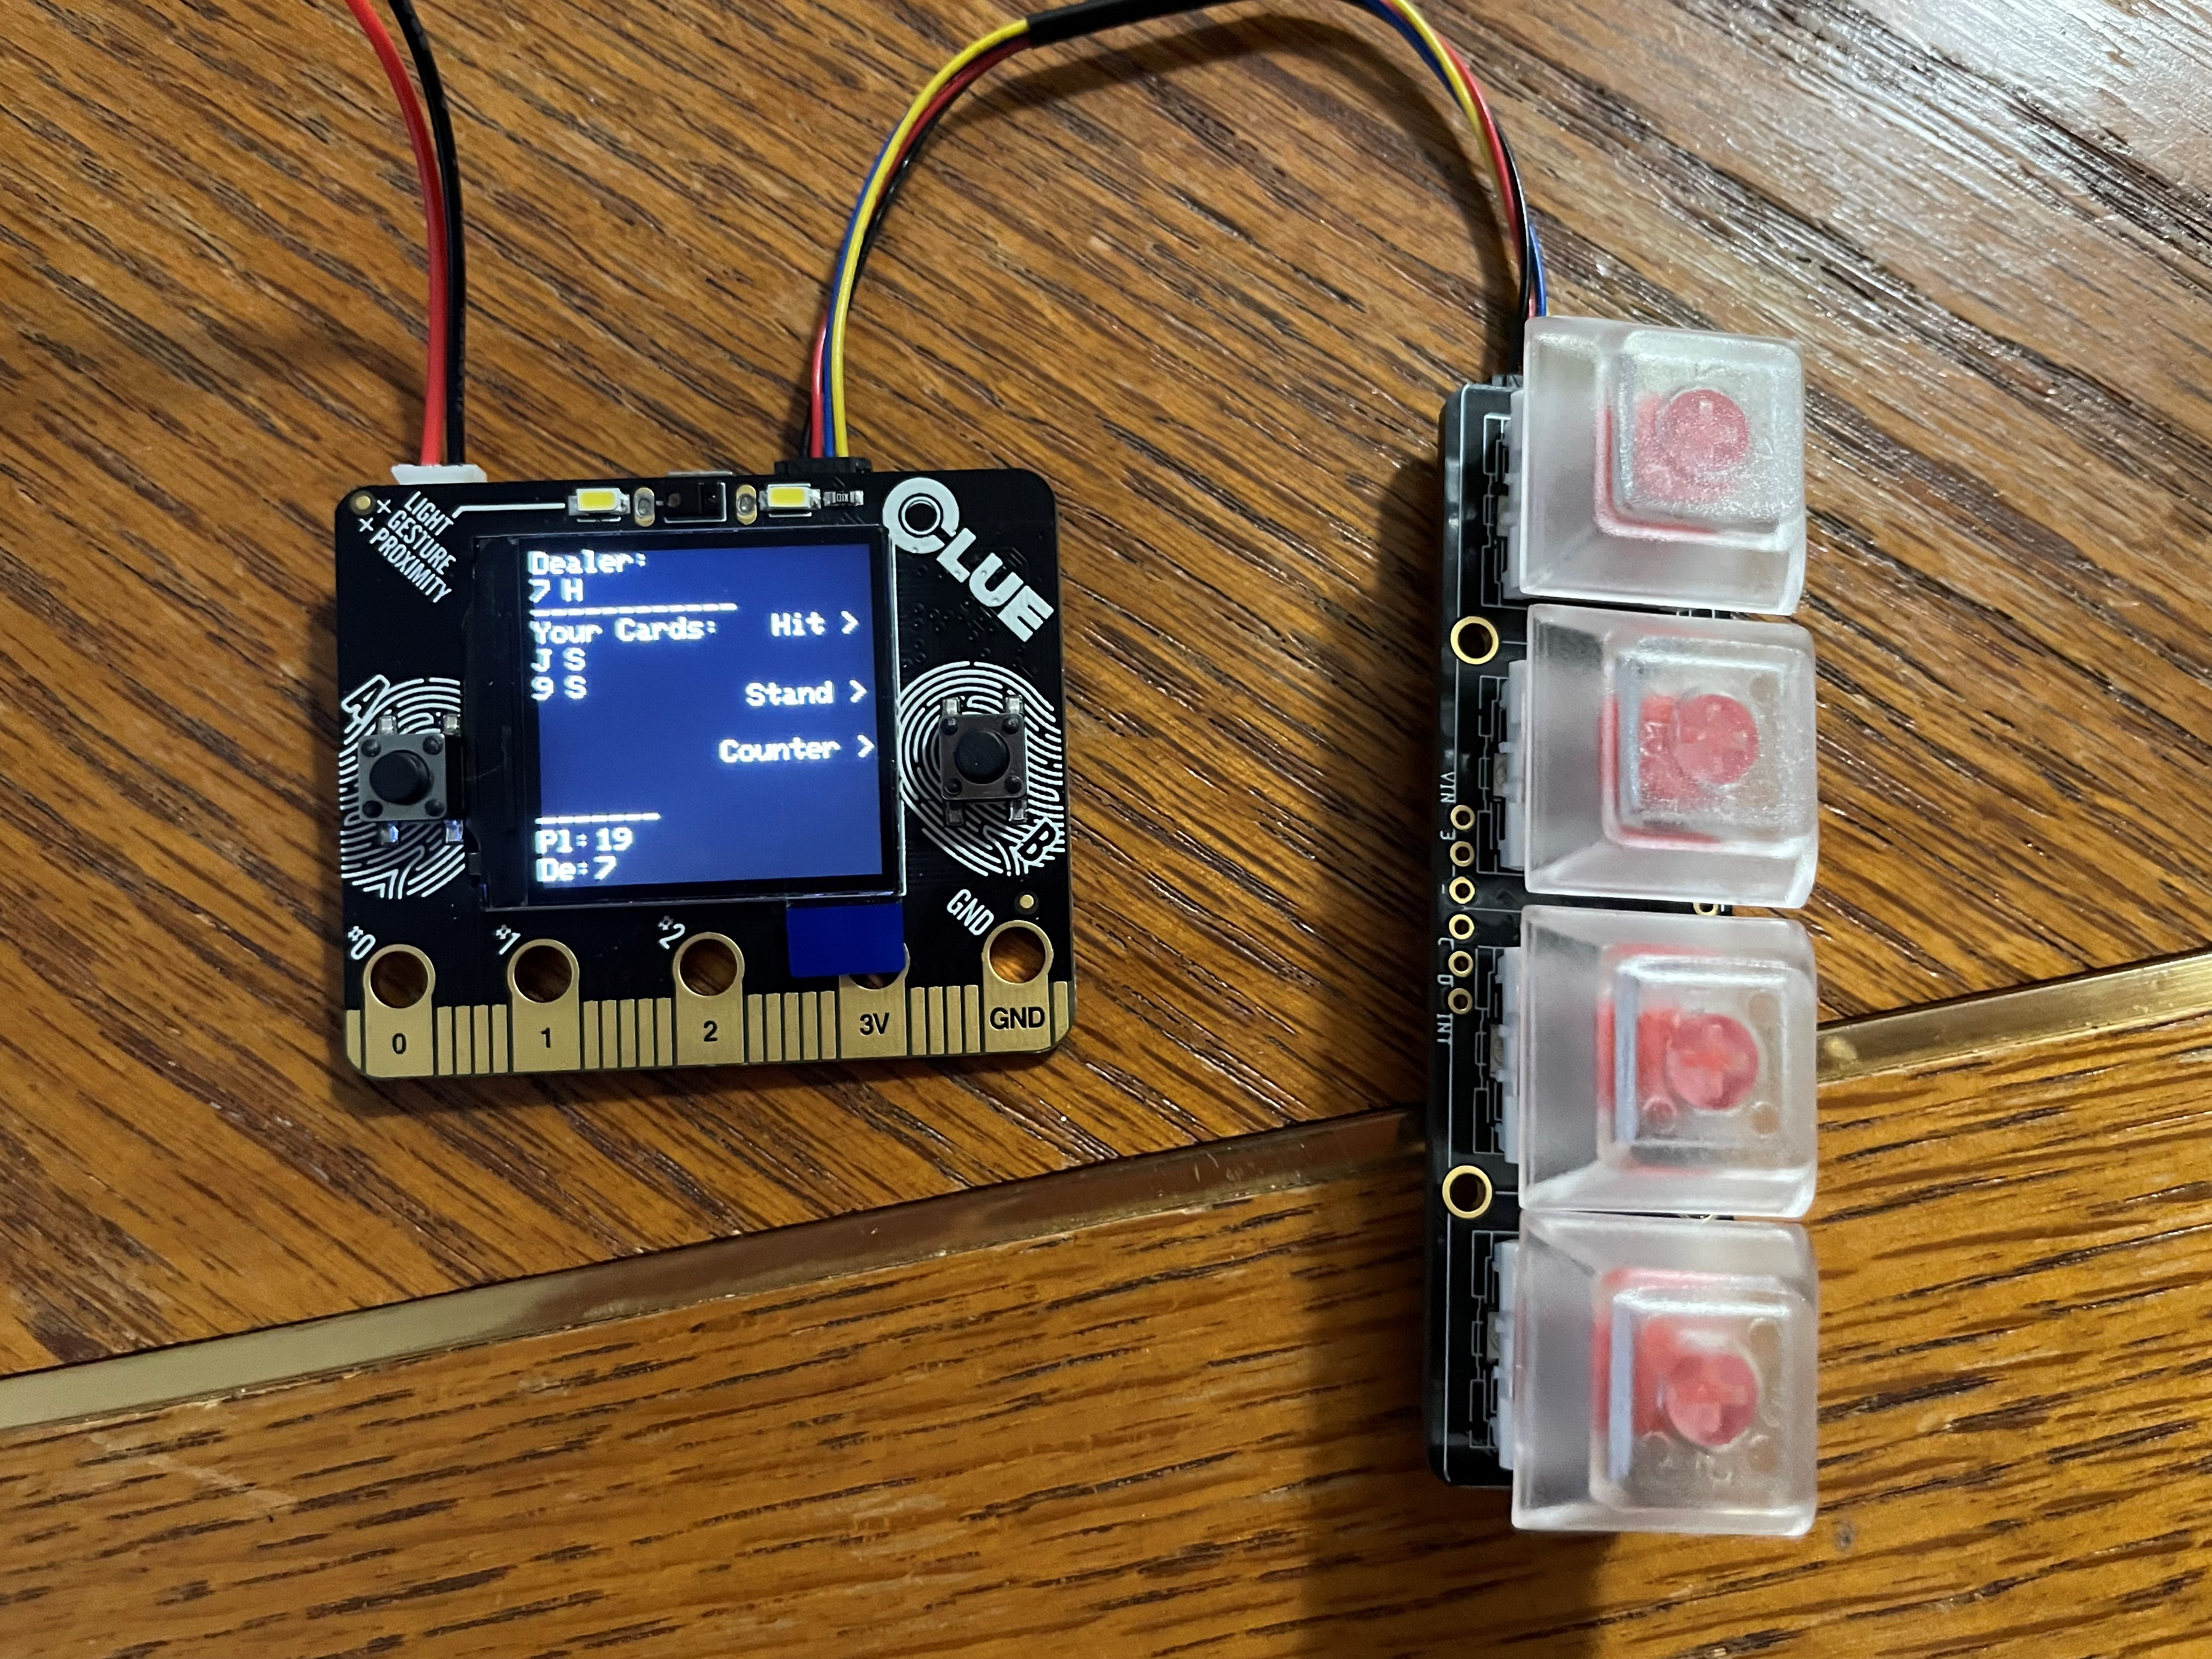
\includegraphics[width=6in]{display.jpg}
  \caption{Display layout on CLUE board}
  \label{fig:display}
  \end{figure}

The card counter on the display can be seen in Figure \ref{fig:counter}.
\begin{figure}[ht]
  \centering
  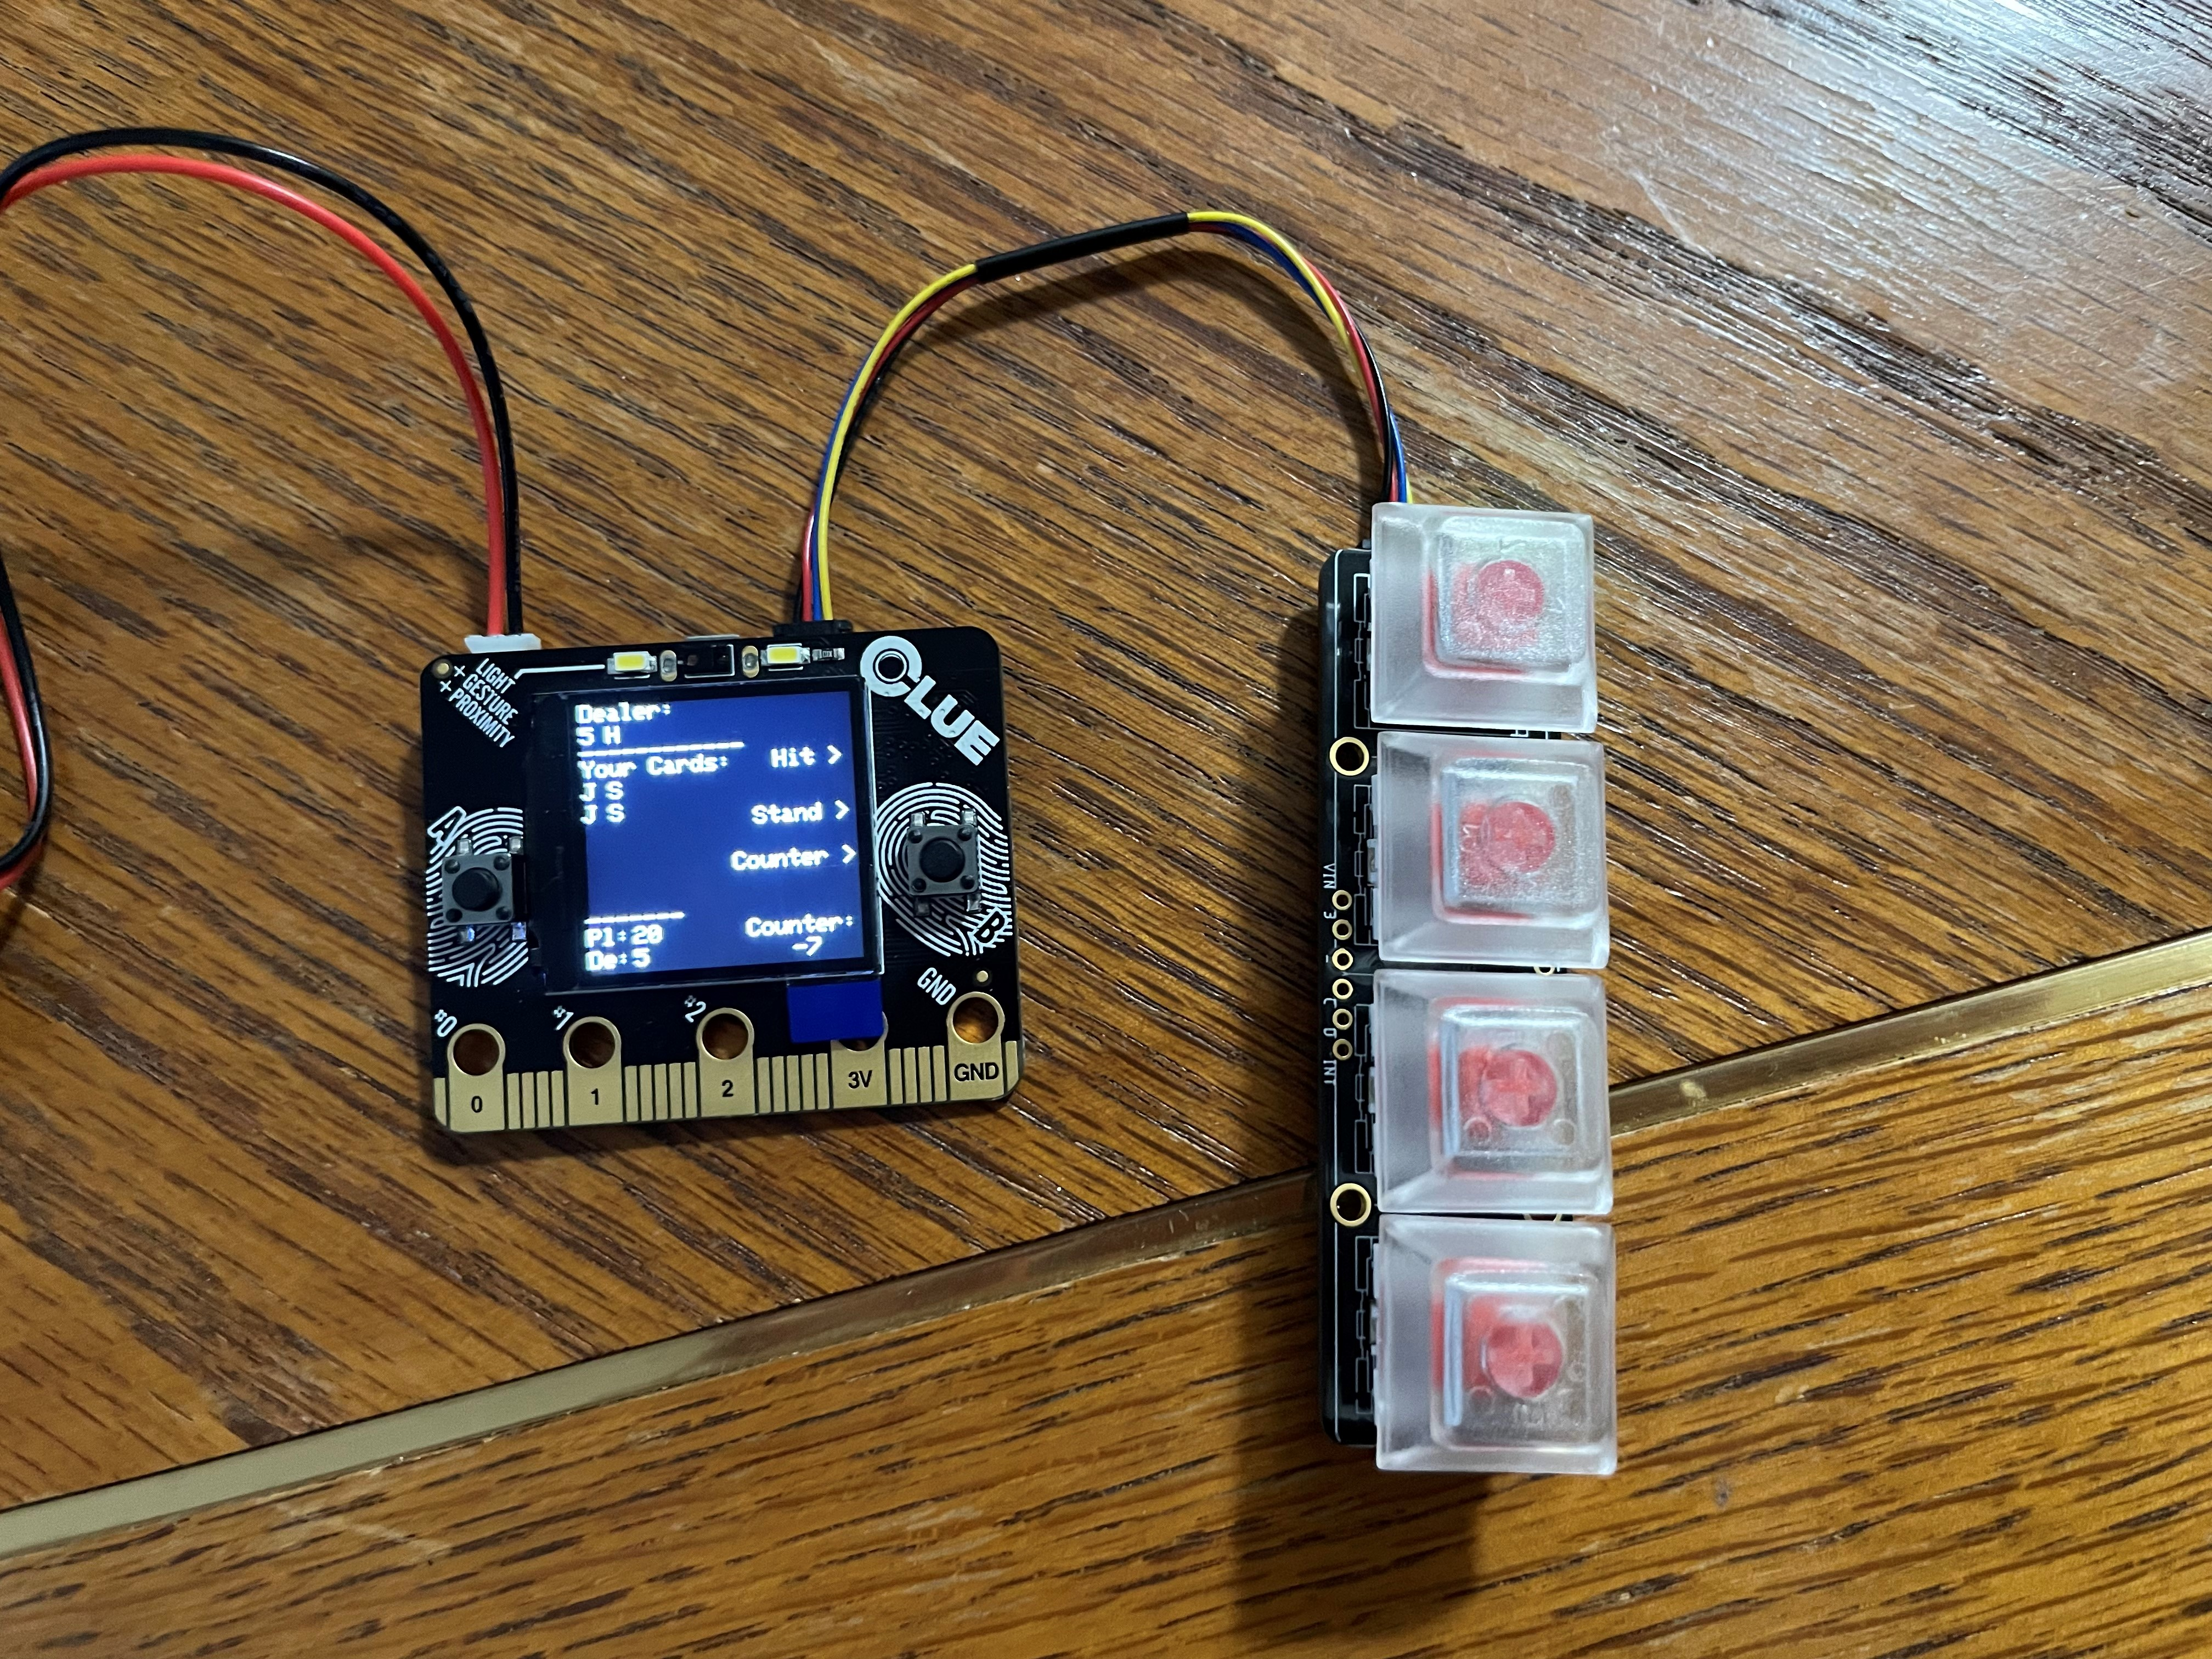
\includegraphics[width=6in]{counter.jpg}
  \caption{Card counter on CLUE board display}
  \label{fig:counter}
  \end{figure}

We first tested the display and button code on the CLUE board by using hard-coded cards, totals, and the card count. This allowed us to make sure the functions were displaying the values passed in correctly. Once the C code was integrated, we were able to check the cards, totals, and count with each other to make sure the correct values were being displayed.

When working with the Neokey board, examples from the Adafruit Seesaw library were used \
Cite{seesaw}. We decided to use the lights on this board rather than the one on the CLUE board due to increased visibility. We also used the top two buttons for the hit and stand actions, and those keys light up when pressed. The hit and stand buttons can be seen in Figures \ref{fig:hit} and \ref{fig:stand}.
\begin{figure}[ht]
  \centering
  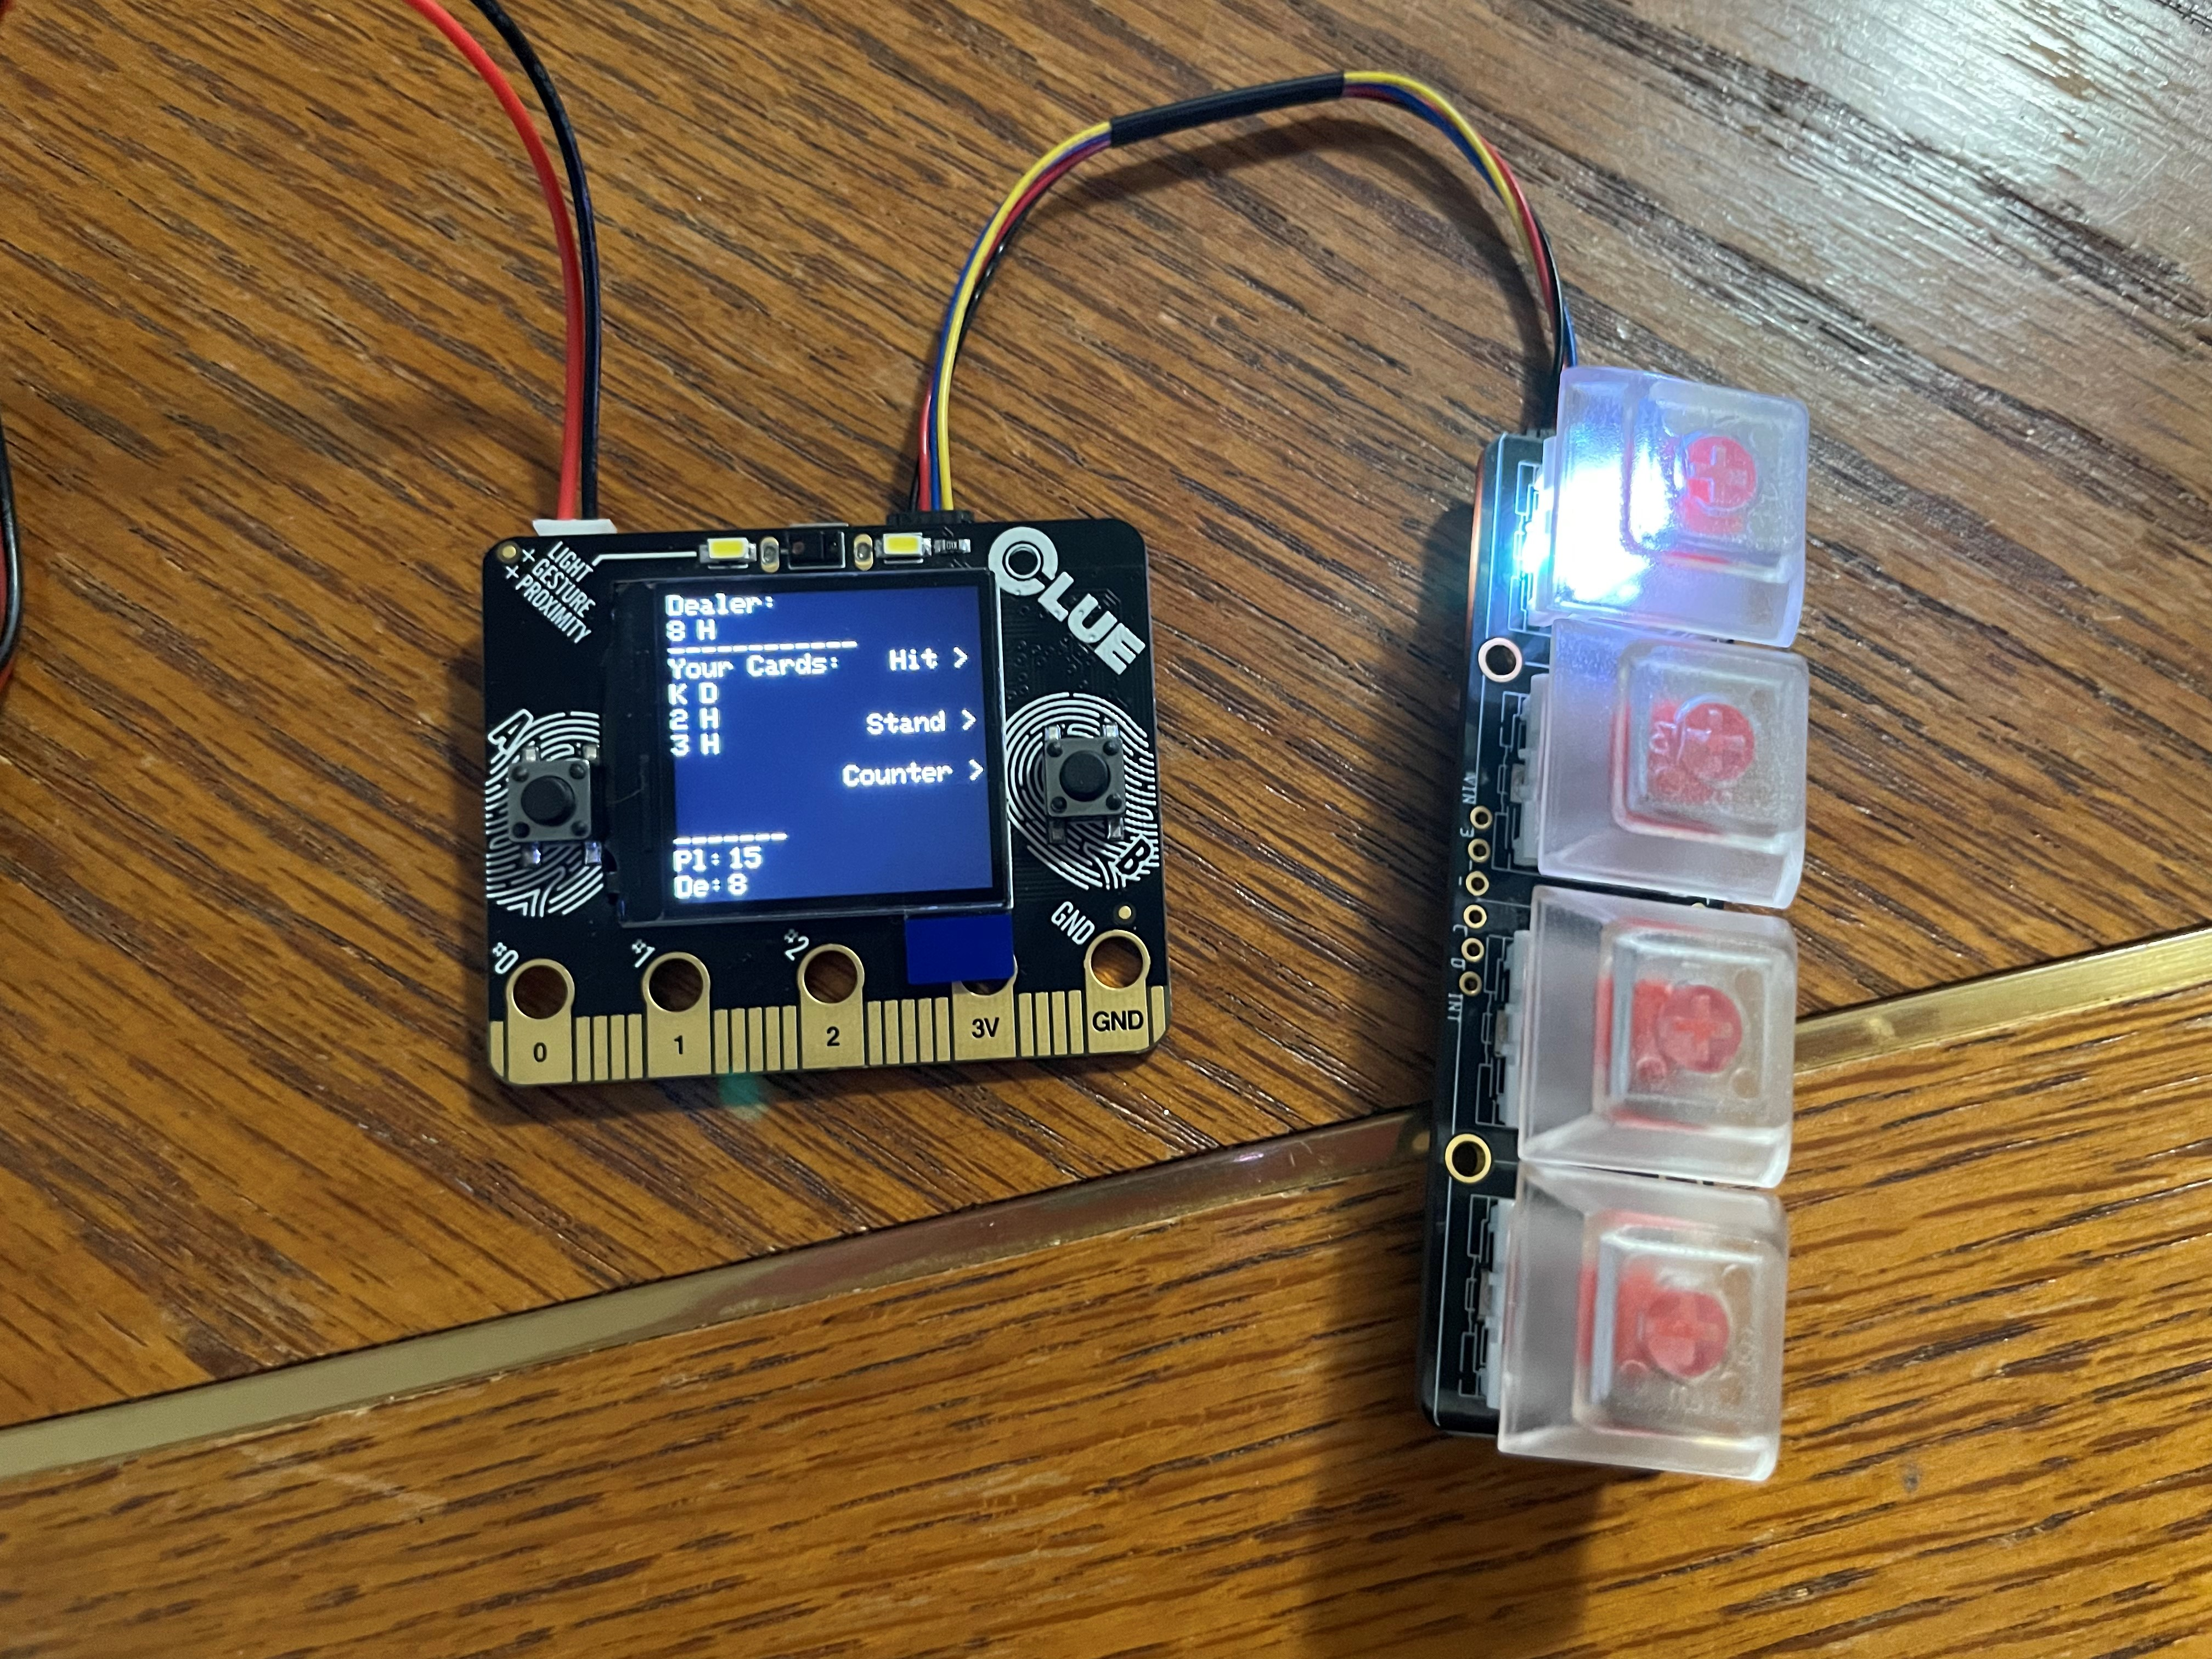
\includegraphics[width=6in]{hit.jpg}
  \caption{Hit key with lights}
  \label{fig:hit}
  \end{figure}

\begin{figure}[ht]
  \centering
  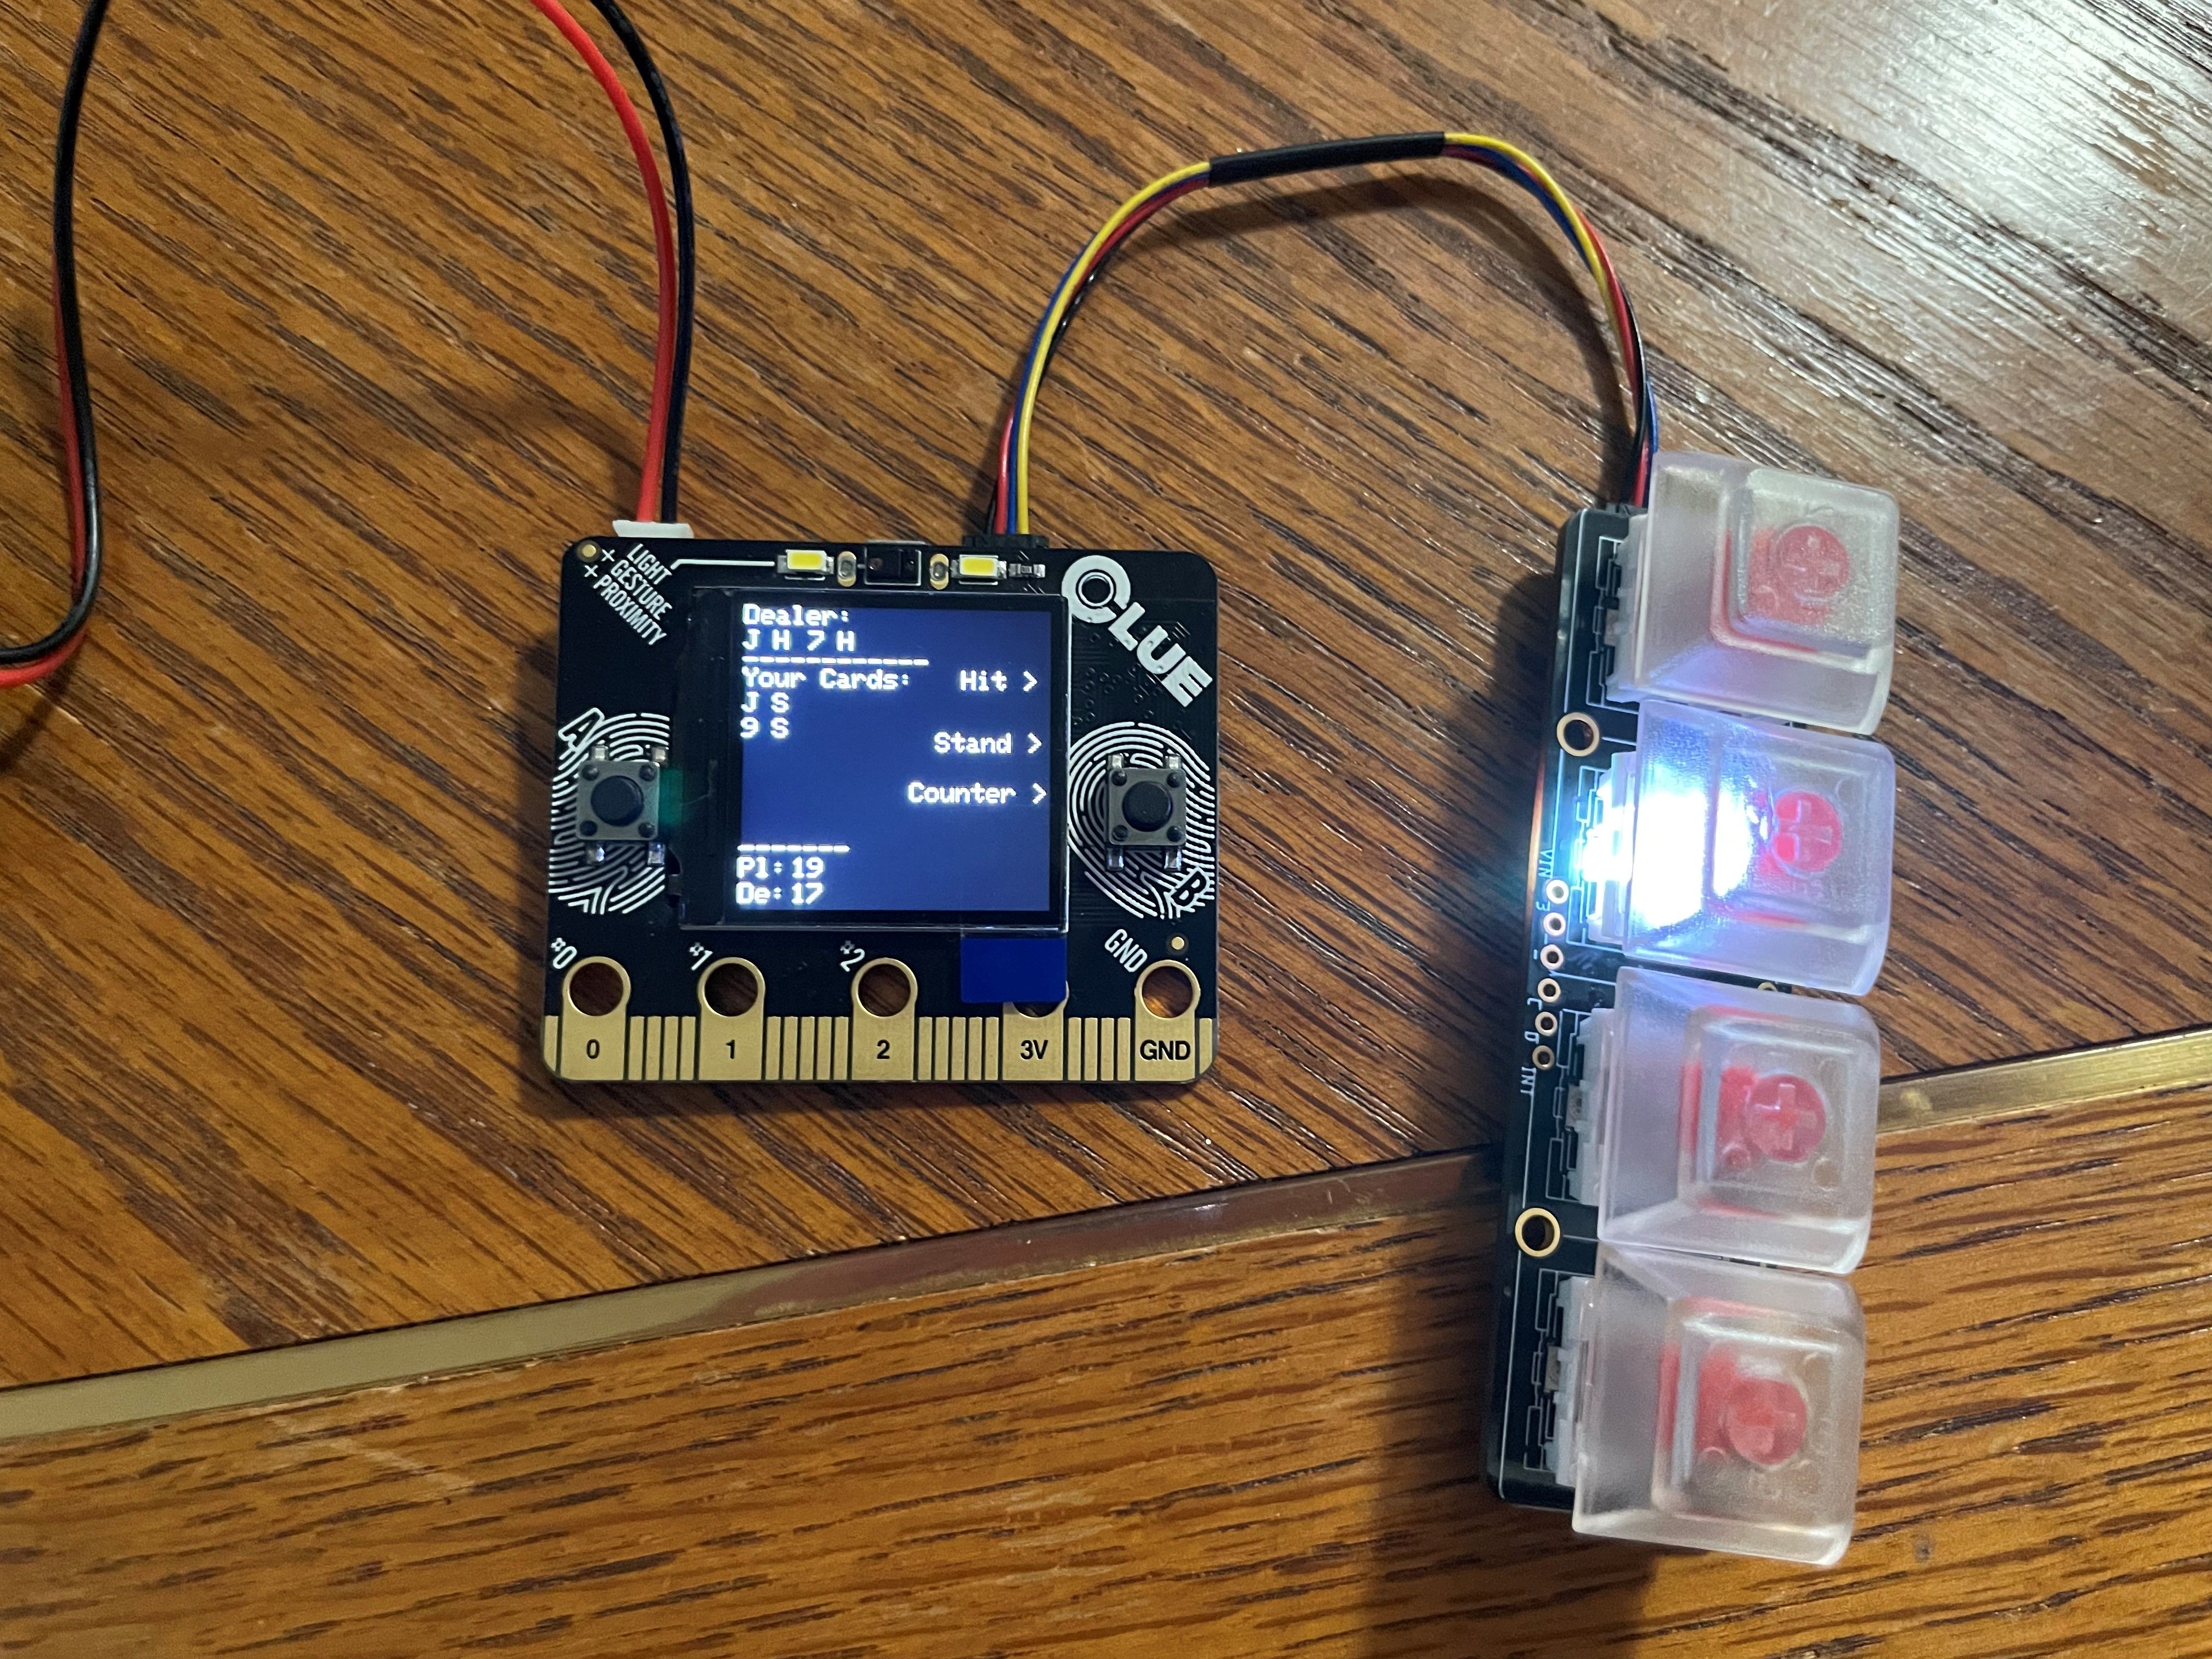
\includegraphics[width=6in]{stand.jpg}
  \caption{Stand key with lights}
  \label{fig:stand}
  \end{figure}

The win/lose scenarios can be seen in Figures \ref{fig:win} and \ref{fig:lose}.
\begin{figure}[ht]
  \centering
  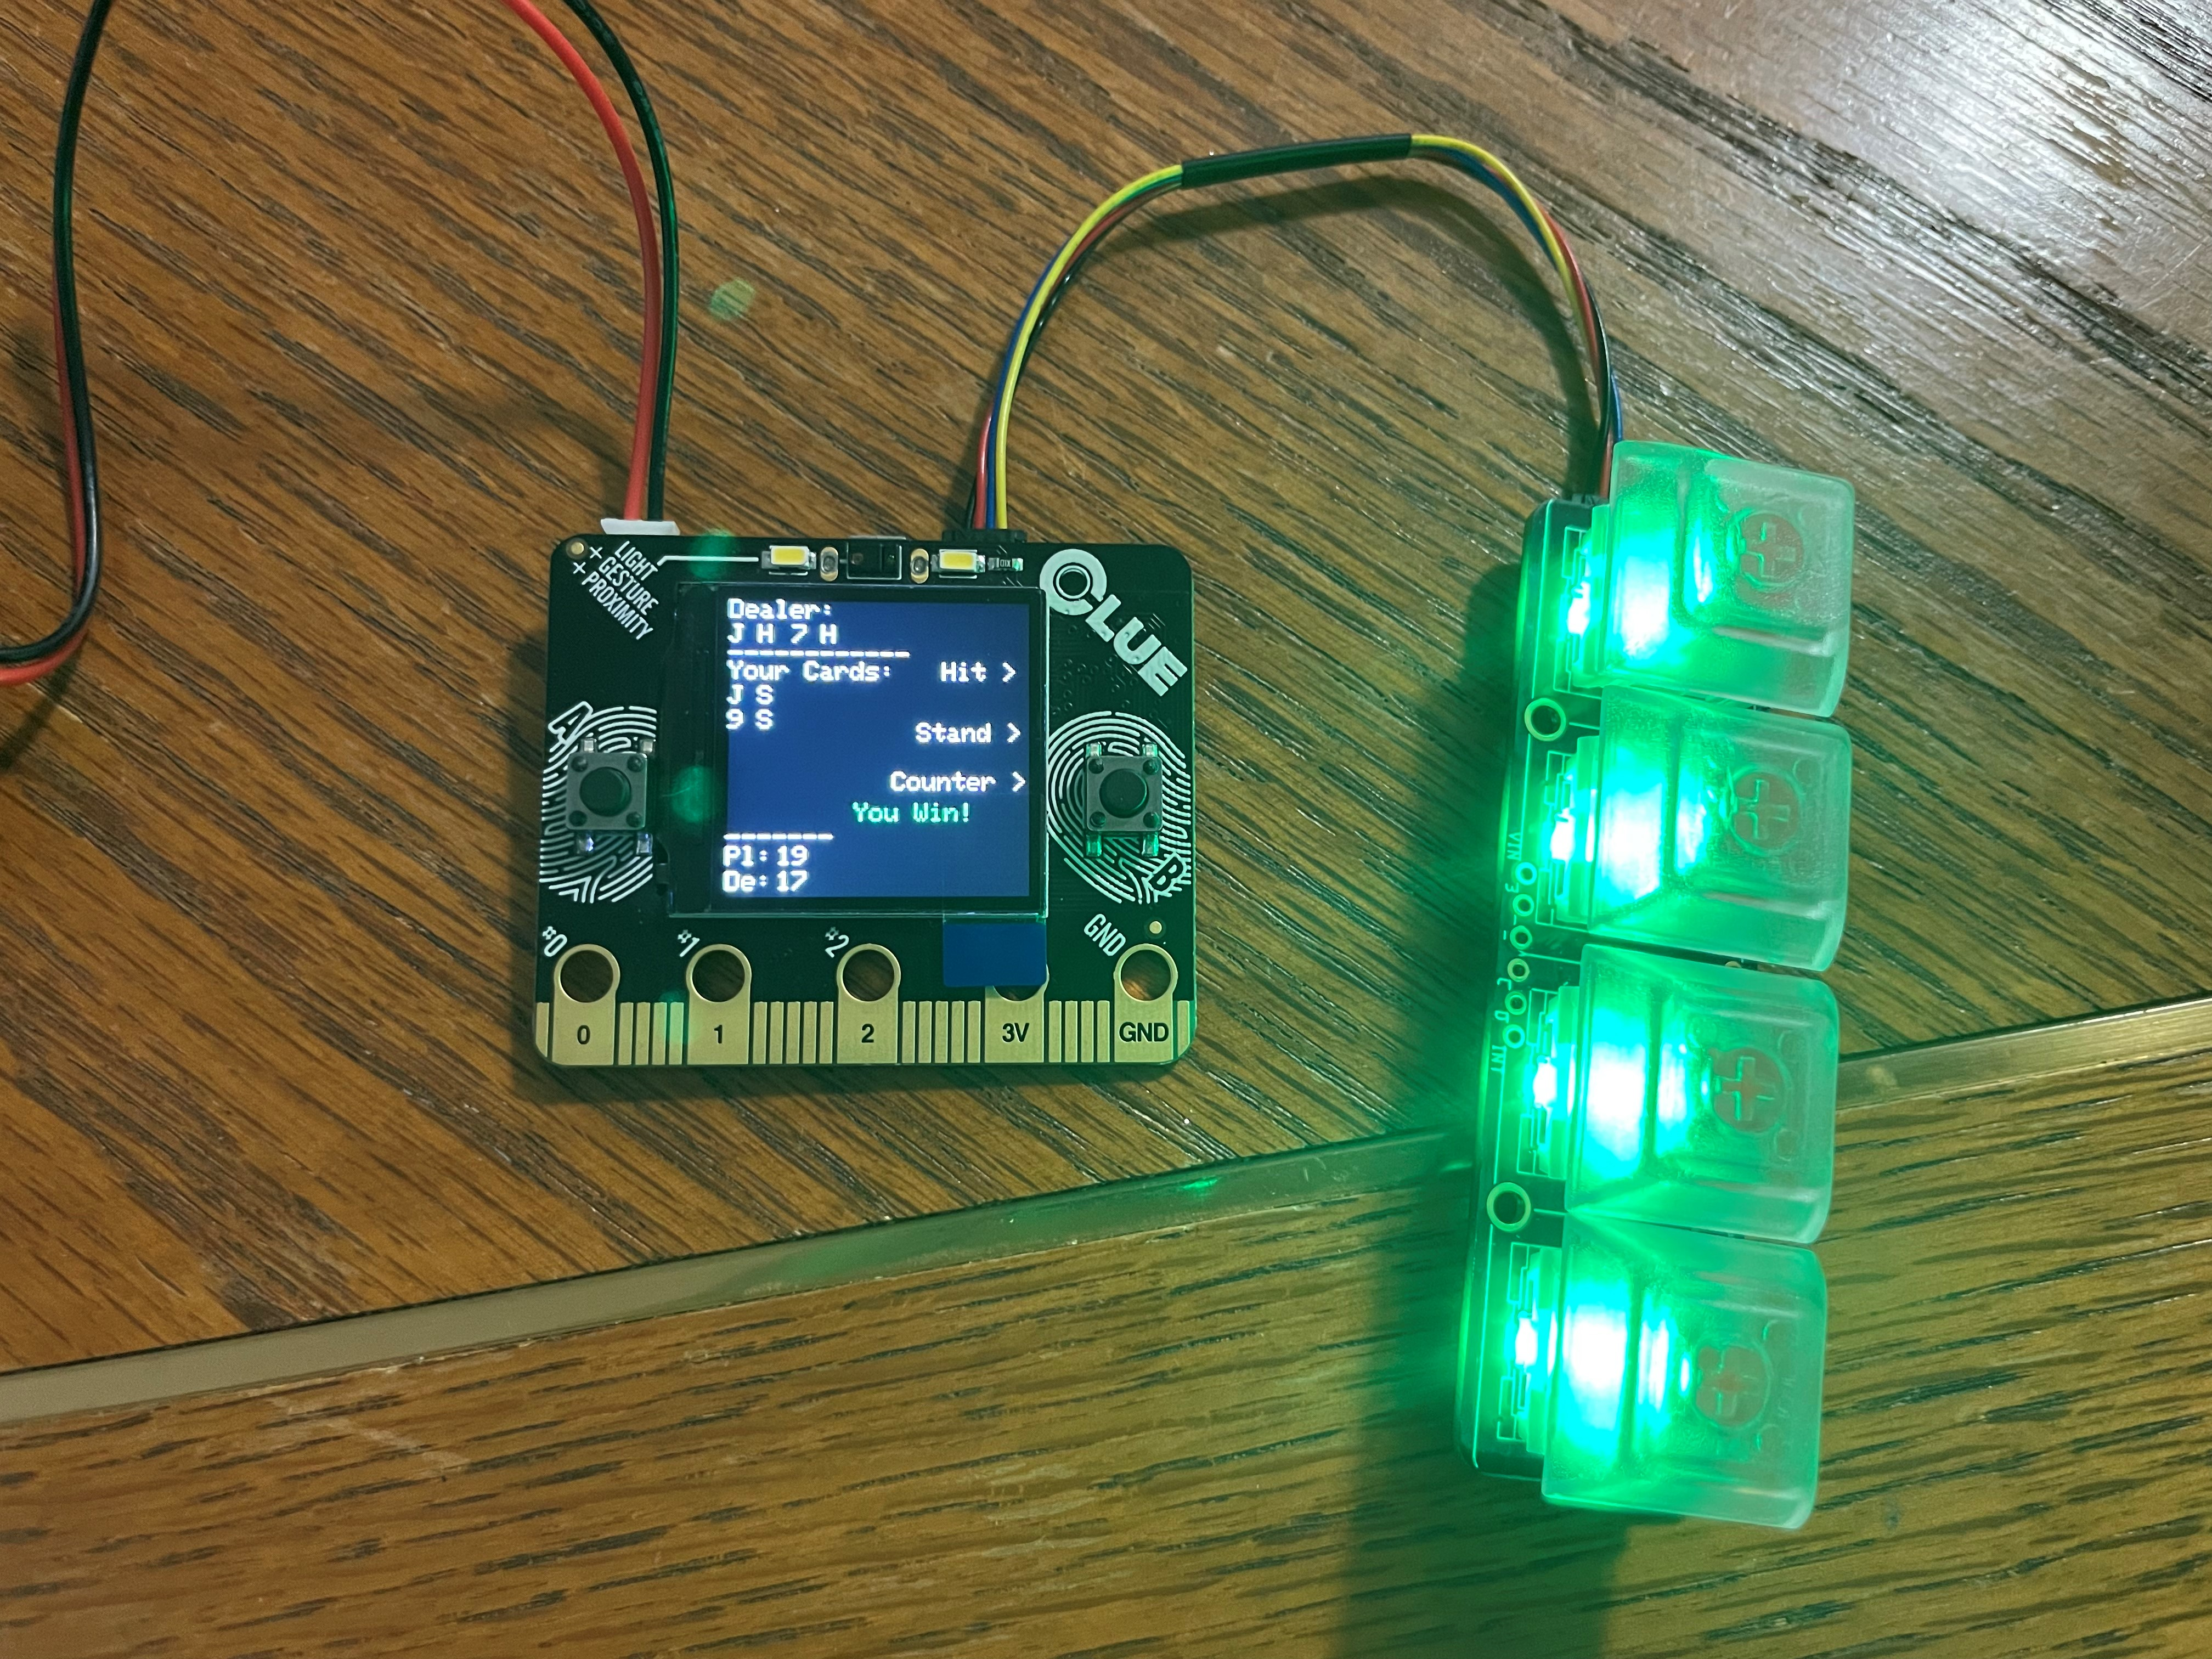
\includegraphics[width=6in]{win.jpg}
  \caption{Win display and lights}
  \label{fig:win}
  \end{figure}

\begin{figure}[ht]
  \centering
  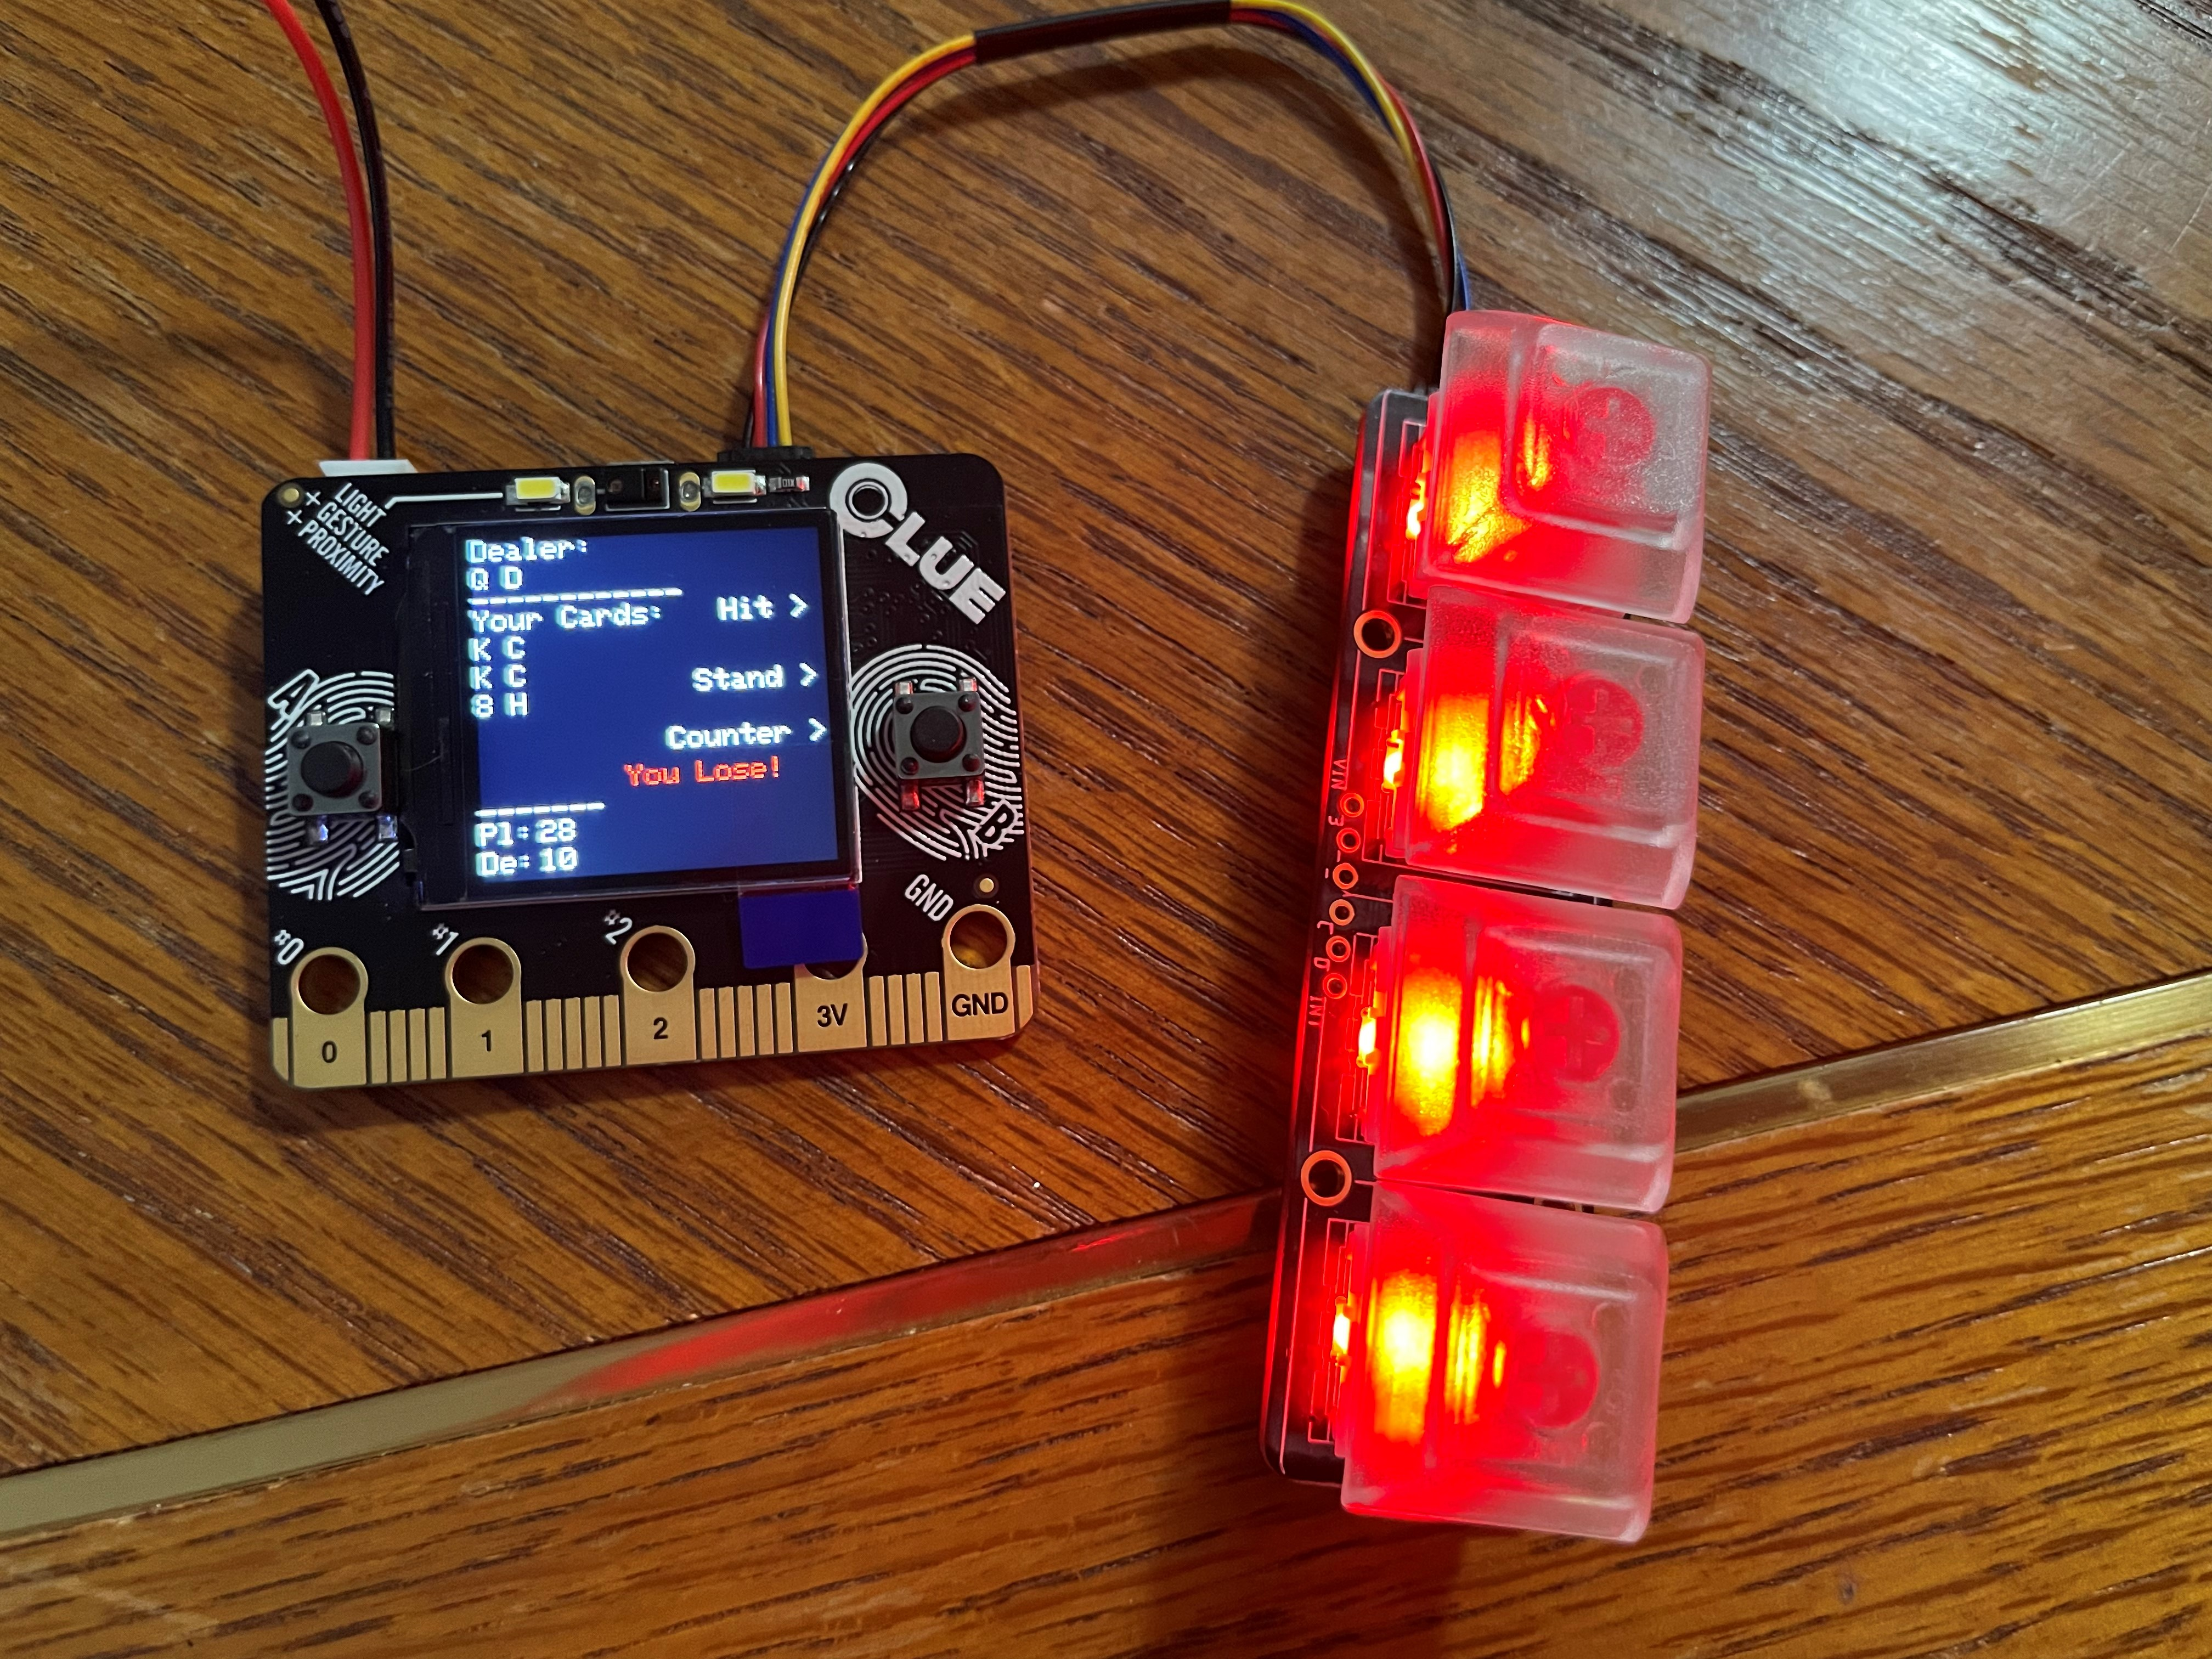
\includegraphics[width=6in]{lose.jpg}
  \caption{Lose display and lights}
  \label{fig:lose}
  \end{figure}

We first tested the display and button code on the Neokey board and for the game-ending conditions by hard coding the win/lose status and by having the buttons on the Neokey board trigger actions like displaying and clearing the card count. This allowed us to check that the lights and buttons were functioning when pressed, and that the win/lose condition on the display matched the lights. Once the C code was integrated, we were able to see how the game played out when each button was pressed and use the totals to check the win/lose conditions with the lights and display. 

We think that the solution with the CLUE and Neokey boards is a good solution. The cards, totals, labels, and counter on the display are clear, as well as the win/lose conditions. The Neokeys are easy to use and it is obvious which button was pressed by the user. The only downside of using the CLUE board that way we did is that the text on the display cannot be appended, so the whole screen must be reset to clear old cards or the card counter.

\section{STATUS}
\subsection{Software}
The project on the side of software development was a complete success. The software is at a point where the game can be played and it can be recognized as Blackjack. Although the basic functions and rules are programmed correctly, it was not possible to get the more advanced functions of the game included within the timeframe allotted for the project. It was one thing to get the game debugged everytime we added a feature, but it was another task to get it integrated successfully with the hardware, which took more time than adding the feature in the first place at times. Due to this abundant amount of time it took to add more functions and rules, we had to sacrifice more advanced features in order to have a working game by the end of the semester.

\subsection{Hardware}
The integration of the NeoKey Buttons and the software into the Adafruit CLUE board was successful and yielded a fully functioning Blackjack game. We achieved a game that played against the dealer with buttons for inputs such as revealing and clearing the card counter, the hit button, and the stand button. In addition, visuals were added to better inform the user if they had won or lost a hand. This was achieved by NeoKey lighting up all red on a loss and all green on a win in addition to a win or lose message displayed on the board. 

Three things that could be worked on would be adding a way to completely exit the game, split logic, and having a random set of card hands. Exiting the game was rather challenging because Arduino runs the main code in an infinite loop. While an attempt was made at writing logic to exit the game, it was unsuccessful, and we chose to direct our efforts towards other issues. The game will also deal a specific set of hands throughout the game and if the CLUE board is reset without a recompile, the same hands will be played over again. We attempted to seed the random number generator to try and change this, however, we did not get it working. We also did not add in the split logic to the hardware because it was not incorporated into the software. Overall, we were able to create a game that a player could play against the computer with a set win or lose scenario.

\subsection{Lessons Learned}
One of the skills our group improved during this project was communication. There was not a lot of time for the project, so we had to divide and conquer between the hardware and software. This required being able to communicate about our code with the other team so that any necessary adjustments or bugs could be fixed. We also had to learn how to find sources for the Adafruit boards, as there are not a lot of resources on how to use the libraries we selected besides the examples. Therefore, we had to be able to pick out the necessary information from the code examples and the header file information to call the classes and functions we needed.

Expanding on the time management, although we did not focus a lot of time on the project over break and before, the last few weeks up until the presentation we were able to effectively set up meetings and split up work to get specific parts of the presentation and code done. Where we could have improved on this was better utilizing the time before break to get most of the initial code done to allow the hardware side more time to convert from C to the arduino and iron out any of the bugs that came with it. Doing this might have allowed us to integrate aspects of the game that were left out of the final version such as splitting and more decks, which would have increased the overall effectiveness of the card counting and simulating a realistic Blackjack game. 

\section{RESULTS}
As our device does not collect data, our only results are reactions from others. Overall, we were complemented by our classmates and instructors on our implementation of the Blackjack game and card counter.

Our Github repository can be found here: \url{https://github.com/Zwalberg/AerE-361-Final-Project}. The code for the project is located in the src folder. The C files contain function declarations, while all of the function bodies and hardware code can be found in Project Hardware Code.ino.

\section{FUTURE WORK}
If we were to continue working on this project, we would implement the split logic into the Blackjack game. The split rule applies at the start of the game; If a player’s starting two cards have the same value, they can decide to split their hand and play on each card as a new hand. We believe this is definitely possible to implement if given more time. The first main issue for this rule’s implementation was that it was hard to build a more advanced game function into an already more advanced game-code structure without breaking what we already had. Another big issue was that this rule changed the display shown to the user, which would have taken a lot of time to build into and debug on the hardware.

Next, we would work on getting the game to have an exit button, ideally on the Neokey board. This would cause the game to stop looping after the current hand ends. We believe this could be done using an if statement to check if the button has been pressed, and if so, the game code is not run in the Arduino loop. We would also work on trying to generate different sets of hands, which we believe may be possible by seeding the random number generator. While we did try this, we didn’t have a lot of time to work with it, and believe more time may solve the issue.

Another addition to the project would be to have a more structured device. As of right now, the clue board and Neokey board are held separately. To increase the player’s experience, it would be beneficial to add a 3D printed case to model a modern day handheld game device. The clear reason for why this was not included up to this point is because it is more important to have a working game rather than improving aesthetics, but we believe it would be feasible given more time. 

\section{CONCLUSION}
The goal of this project was to create a functioning game of Blackjack with a card counter with the intent to teach new players not only how to just play the game but to teach them how to play in a way that increases their odds of winning. Although some high-level functions had to be left out of the current version of the game, we believe that the project was a success in the aspect of what was accomplished within the given timeframe. 

A lot was accomplished during this project, but even more was learned. There were a lot of unknowns going into the project on both the software and hardware side. The group was able to play to each other’s strength and learn new things in order to accomplish a common goal. 

\newpage

\printbibliography[heading=subbibintoc]
\newpage
% you need to have at least your code in your appendix
\appendix

\section{SOURCE CODE}
\lstinputlisting[language=Arduino]{../../Firmware/src/ProjectHardwareCode.ino}
\end{document}